%\documentclass[aps,prd,nofootinbib,amsmath,notitlepage]{revtex4-1}
\documentclass[11pt]{article}
\usepackage{jcappub}
\usepackage{amssymb,esvect,amsmath,graphicx,latexsym,amsthm,slashed,eso-pic,fullpage}
\usepackage[final]{pdfpages}
\usepackage{array}
\usepackage{soul}
\usepackage[normalem]{ulem}
\usepackage{multirow}
\usepackage{pbox}
\DeclareMathOperator{\ev}{eV} \DeclareMathOperator{\kev}{KeV} \DeclareMathOperator{\mev}{MeV} \DeclareMathOperator{\gev}{GeV} \DeclareMathOperator{\tev}{TeV} \DeclareMathOperator{\cm}{cm} \DeclareMathOperator{\barn}{barn} \DeclareMathOperator{\g}{g} \DeclareMathOperator{\km}{km} \DeclareMathOperator{\pb}{pb} \DeclareMathOperator{\s}{s} \DeclareMathOperator{\yr}{yr}\DeclareMathOperator{\gyr}{Gyr} \DeclareMathOperator{\kg}{kg} \DeclareMathOperator{\mpc}{Mpc} \DeclareMathOperator{\few}{few} \DeclareMathOperator{\kel}{K}
\newcommand{\cA}{{\cal A}} \newcommand{\cC}{{\cal C}} \newcommand{\cD}{{\cal D}} \newcommand{\cE}{{\cal E}} \newcommand{\cF}{{ \cal F}} \newcommand{\cH}{{\cal H}} \newcommand{\cJ}{{\cal J}} \newcommand{\cL}{{\cal L}} \newcommand{\cM}{{\cal M}} \newcommand{\cN}{{\cal N}} \newcommand{\cO}{{\cal O}} \newcommand{\cP}{{ \cal P}} \newcommand{\tp}{{ \tilde p}} \newcommand{\cR}{{\cal R}} \newcommand{\cS}{{\cal S}}
\newcommand{\ep}{\epsilon} \newcommand{\vp}{\varphi} \newcommand{\half}{\frac12}
\newcommand{\ie}{{\it i.e.~}}  \newcommand{\eg}{{\it e.g.~}}
\newcommand{\pt}{\partial} \def\d{{\rm d}}  \def\oL{\overline} \def\wh{\widehat}
\newcommand{\pL}{\left(} \newcommand{\pR}{\right)} \newcommand{\bL}{\left[} \newcommand{\bR}{\right]} \newcommand{\cbL}{\left\{} \newcommand{\cbR}{\right\}} \newcommand{\mL}{\left|} \newcommand{\mR}{\right|} \newcommand{\ER}{E_R}
\newcommand{\beq}{\begin{equation}} \newcommand{\eeq}{\end{equation}}
\newcommand{\bea}{\begin{eqnarray}} \newcommand{\eea}{\end{eqnarray}}
\newcommand{\alg}[1]{\begin{align} \begin{split} #1 \end{split}  \end{align}}
\newcommand{\vev}[1]{\langle {#1} \rangle}
\newcommand{\tenx}[1]{\times 10^{#1}}
\newcommand{\Eq}[1]{Eq.~(\ref{#1})} \newcommand{\Eqs}[2]{Eqs.~(\ref{#1}) and (\ref{#2})} \newcommand{\Eqm}[2]{Eqs.~(\ref{#1}) through (\ref{#2})}
\newcommand{\Sec}[1]{Sec.~\ref{#1}} \newcommand{\Secs}[2]{Secs.~\ref{#1} and \ref{#2}} \newcommand{\Secm}[2]{Secs.~\ref{#1} through \ref{#2}}
\newcommand{\Fig}[1]{Fig.~\ref{#1}} \newcommand{\Figs}[2]{Figs.~\ref{#1} and \ref{#2}}
\newcommand{\Tab}[1]{Tab.~\ref{#1}}
\newcommand{\App}[1]{App.~\ref{#1}}
\DeclareMathOperator{\br}{Br} \DeclareMathOperator{\tr}{Tr}
\newcommand{\arxiv}[1]{{\href{http://arxiv.org/abs/#1}{\tt #1}}}

\newcommand{\sdm}[1]{\textcolor{blue}{\textbf{(#1 -- SDM)}}}

\newcommand{\sjwColor}{red}
\newcommand{\sjw}[1]{{\color{\sjwColor} #1}}
\newcommand{\sjwrm}[1]{{\color{\sjwColor}\protect\sout{#1}}}
\newcommand{\sjwrp}[2]{\sjwrm{#1} \sjw{#2}}
\newcommand{\sjwtt}[1]{{\color{\sjwColor}\tt #1}} 

\begin{document}
\title{Model Selection with a Single Target:\\Leveraging Annual Modulation to Differentiate Direct Detection Signals}
\author[a,b]{Samuel J.~Witte,}
\author[c]{Vera Gluscevic, and}
\author[d]{Samuel D.~McDermott}


\affiliation[a]{University of California, Los Angeles, Department of Physics and Astronomy, Los Angeles, CA 90095}

\affiliation[b]{Fermi National Accelerator Laboratory, Center for Particle
Astrophysics, Batavia, IL 60510}

\affiliation[c]{School of Natural Sciences, Institute for Advanced Study, Einstein Drive, Princeton NJ 08540, USA}

\affiliation[d]{C.~N.~Yang Institute for Theoretical Physics, Stony Brook, NY, USA}\subheader{\rm YITP-SB-16-NN}

\abstract{


}

\maketitle

\section{Introduction} \setcounter{page}{2}

Experimental evidence from a vast array of independent sources conclusively demonstrates the existence of a non-baryonic form of matter in the universe. This so-called dark matter is the dominant source of the gravitational potential wells that have determined the large scale structure of the universe, but dark matter particles have yet to be observed in a laboratory setting. Despite an experimental direct detection program that has now been mature for several decades, all evidence in favor of the existence of dark matter is instead furnished by indirect observations of cosmological and astrophysical settings \sjwtt{potentially cite something? maybe : e.g. see X for review of direct detection}.

There are good reasons to be optimistic that direct detection may be on the cusp of important discoveries, however. As next-generation experiments that incorporate increasingly precise detection technologies come online, we will be pushing through the final parameter space before encountering the astrophysical neutrino background \sjwtt{additional citations? -- most of the ones listed discuss consequences of neutrino floor -- may be worth citing future reach potential papers for Xenon1T, LZ, superCDMS, etc.}\cite{Cushman:2013zza,Billard:2013qya,Ruppin:2014bra,Davis:2014ama,Dent:2016iht}. Luckily, many interesting theories of dark matter predict scattering cross sections in this range. For example, heavy $SU(2)$-doublet and -triplet fermions, such as the Higgsinos and the wino of supersymmetry, are expected to have cross sections of order $\sigma_{\rm SI} \sim \cO(\few\tenx{-48})\cm^2$, fixed by their Standard Model gauge quantum numbers alone \cite{Hill:2011be,Hill:2013hoa,Hill:2014yxa}, while a heavy $SU(2)$-singlet fermion, like the bino, is around an order of magnitude lower depending on its coannihilation partner \cite{Berlin:2015njh}. Models with kinematically suppressed tree-level scattering may also be embedded in more complete dark sectors that have loop-level cross sections in this same range \cite{Ipek:2014gua,McDermott:2014rqa,Appelquist:2015yfa,Appelquist:2015zfa}.

Because so many theories can be accommodated in the parameter space that we will imminently probe, we must plan for the science opportunities associated with the first detection of dark matter particles. The ``inverse problem'' that we will confront upon successful detection of dark matter particles is that of understanding the (high-energy) dark sector dynamics solely by examining (low-energy) recoils of detector elements. \sjwrm{In collider physics terms, the luminosity is fixed by the dark matter astrophysics, making measurements of dark matter properties possible only at a single energy scale.} \sjwtt{I don't really know what this adds... I find its presence rather confusing} We will need to reconstruct the interesting physics of the dark sector at all scales from nuclear recoils alone, despite the fact that the details of the dynamics that link the dark sector to the Standard Model are most likely integrated well above the low energies probed in direct detection experiments. On the other hand, because the dynamics are coarse grained at the energies of direct detection experiments, the nuclear responses are compactly described by an easily exhaustible list of interactions. These are collected as a nonrelativistic effective field theory \cite{Fitzpatrick:2012ix, Anand:2013yka}. This ``effective field theory of dark matter direct detection'' reproduces the nontrivial nuclear physics induced by some of the best-motivated UV-complete theories of dark matter \cite{Gresham:2014vja, Gluscevic:2015sqa}. %As described presently, we can look for clues to the nature of the dark sector along two orthogonal axes with the help of this effective theory.
All of the characteristic information about the dark sector interactions is contained in the coefficients of the effective theory. The key to accessing this information and unlocking the secrets of the dark matter interactions lies in the careful study of the scattering data in the event of a detection.

Much of the information one might hope to access from a direct detection experiment is contained in the energy spectra of nuclear or electronic recoils. Due to Poisson noise and degeneracies in the spectra of different interactions, model selection using spectral information alone is difficult with a single target material. However, recent studies show it is possible to discriminate between interactions by leveraging the energy spectra from nuclei with sufficiently diverse nuclear physics characteristics. Thus, energy spectra of experiments with different nuclei can break degeneracies in the dark matter model space, as long as the target nuclei have ``complementary'' nuclear physics characteristics \cite{McDermott:2011hx,Peter:2013aha,Gluscevic:2014vga,Catena:2014epa,Catena:2014hla,Dent:2015zpa,Gluscevic:2015sqa,Ruppin:2014bra}.

In this work, \sjwrm{we will the dark sector from low-energy physics:} we will show that information from the time distribution of scattering events also helps break \sjw{model} degeneracies \sjwrm{in model space}. Almost since the dawn of the study of direct detection experiments, the annual modulation of the rate \cite{Freese:1987wu} arising from the motion of Earth relative to dark matter bound in the galactic halo has been appreciated to provide a distinctive dark matter signature, as have its higher harmonics (see e.g. \cite{Freese:2012xd,Lee:2013xxa,Britto:2014wga,DelNobile:2015nua,Kouvaris:2015xga}). \sjw{ The disturbance of phase space from nonstandard astrophysics \cite{Green:2000ga,Gelmini:2000dm,DelNobile:2015nua} and the gravitational influence of the solar system \cite{Lee:2013wza,DelNobile:2015nua} have been shown to a non-negligible impact on the annual modulation. }\sjwtt{After messing with the above sentence a few times I've decided I don't know why its there. We never address dark matter substructure or non-standard astrophysical contributions -- they inevitably make the analysis WAY harder, why are we mentioning this? GF discussion can wait til later, its a higher order effect.} \sjwrm{Later, it was pointed out that similar effects are produced from nonstandard particle physics models}\sjwtt{The above sentence is not exactly correct. The below sentence is a more appropriate sentence, although I'm not sure this belongs here. I think perhaps we should hold off on this until we discuss $v^\perp$ dependence.}\sjw{While it is typically assumed that properties of the modulation are determined solely by astrophysical processes, it was recently pointed out in~\cite{DelNobile:2015tza,DelNobile:2015rmp} that a particular class of dark matter-nuclei interactions can produce a modulation that is unique to each target element}. Here we will demonstrate that even within classes of interactions with approximately degenerate recoil spectra the additional discrimination power from timing information will allow some of the most popular detector designs to go beyond detection and significantly improve model identification. \sjwrm{In this way, it may be possible to discriminate between certain models of the dark matter using a single detector element on its own.}\sjwtt{ perhaps not entirely true...}


In \Sec{sec:dd} we review the calculation of the direct detection scattering rate. \Sec{sec:eft} introduces the concept of dark matter effective field theory, discusses how momentum and velocity dependent cross sections can result in nonstandard scattering, and reviews dark matter models which have nearly degenerate recoil spectra but distinguishing time dependence. We introduce our analysis procedure in \Sec{sec:procedure} and present our results in \Sec{sec:results}. We conclude in \Sec{sec:conclusion}.


  

\section{Dark Matter Direct Detection: Energy and Time Dependence}\label{sec:dd}

The observed recoil energy spectrum is the number count of nuclear recoil events observed per recoil energy $E_R$, per unit time, per unit target mass,
\begin{equation}
\frac{dR}{dE_R dt}(E_R,t) =  \frac{\rho_\chi}{m_T m_\chi} \int\limits_{v_{\mathrm{min}}}^{v_{\mathrm{esc, lab}}}  v f(\mathrm{\mbox{\bf{v}}}|t) \frac{d\sigma_T}{dE_R} (E_R,v) d^3v ,
\label{eq:dRdEr_general}
\end{equation}
where:
\begin{itemize}
\item $\rho_\chi$ and $m_\chi$ are the local dark matter density and the dark matter particle mass
\item $v_\mathrm{min} = \sqrt{m_T E_R/2\mu_T^2}$ \sjw{only for elastic scattering} is the minimum velocity a dark matter particle of mass $m_\chi$ needs to produce a nuclear recoil of energy $E_R$, where $\mu_T=\frac{m_Tm_\chi}{m_T+m_\chi}$ is the reduced mass of the dark matter particle and the target nucleus
\item $v_{\mathrm{esc, lab}}$ is the escape velocity from the Galactic halo in the lab frame
\item $v$ is the velocity of the dark matter in the lab frame
\item $f(\mathrm{\mbox{\bf{v}}}|t)$ is the observed dark matter velocity distribution, which is generically time-dependent
\item and $d\sigma_T/dE_R=m_T \sigma_T /2\mu_T^2 v^2$ is the differential cross section for dark matter scattering off a target \sjw{nuclide T}; \sjwrm{in this work, we focus on nuclear recoils, and we focus on the physics of $d\sigma_T/dE_R=m_T \sigma_T /2\mu_T^2 v^2$ in the next section }\sjwtt{I don't think this last part is necessary to include here}.
\end{itemize}


The differential rate in \Eq{eq:dRdEr_general} is determined by the experimental setup, the dark matter astrophysics, the particle properties of dark matter, the nuclear properties of the target material $T$ (throughout this paper we use $T$ to denote the nuclear target and we reserve $N$ to denote a nucleon, either $n$ or $p$), and the dark matter-nuclei interaction. For the purposes of this study, we set the astrophysical parameters to the following values \cite{Bovy:2013raa,Piffl:2013mla}: $\rho_\chi=0.3$ GeV/cm$^3$; $v_{\mathrm{esc}} = 533$ km/sec in the Galactic frame; we assume that $f(\mathrm{\mbox{\bf{v}}})$ is a Maxwellian distribution in the Galactic frame, with an rms speed of $155$ km/sec, and a mean speed equal to the Sun's rotational velocity around the Galactic center, $v_\textrm{lag}=220$ km/sec. The underlying particle physics model determines the calculation of the recoil rate through the differential scattering cross section ${d\sigma_T}/{dE_R}$, as discussed in \cite{Gluscevic:2015sqa,Gresham:2014vja}: this has a free normalization with units of cm${}^2$ as well as a discrete set of functional dependences on $E_R$ and $v$.


The total rate $R$ of events is the integral of the differential rate within the nuclear-recoil energy range $\cE$ of a given experiment\footnote{For simplicity, in this work we assume unit efficiency of detection, at all energies within the analysis window, for each experiment considered here, and rescale the exposures to take this assumption into account when choosing experimental parameters to represent the capabilities of Generation 2 (Gen2) experiments.}, $R(t)=\int_\cE \frac{dR}{dE_R dt} dE_R$. In turn, the total expected number of events $N$ for a target of total mass $\cM$ from a time $t_1$ to $t_2$ over $\cE$ is
\beq
N =  \cM \int\limits_{t_1}^{t_2} \int\limits_\cE  \frac{dR}{dE_R dt}(E_R,t)\,dE_R \,dt.
\eeq
\sjw{I dont think  we should have this paragraph below. Obviously the total number of events is important, but our entire discussion on Bayesian model selection is left to a later section. }The total number of events and the differential rate for a given energy and time will be used to define a likelihood function. This likelihood can be interpreted as a function of particle physics inputs, which in turn parameterize a posterior probability distribution. The integral over this posterior will finally provide a Bayesian evidence in favor of a particular model. Comparing evidence from different particle physics models allows model selection as described in \cite{Gluscevic:2014vga, Gluscevic:2015sqa}.



As is clear in \Eq{eq:dRdEr_general}, the differential rate of nuclear recoils depends on time. This arises from the motion of the earth about the sun. In the galactic rest frame, the dark matter is thought to be well approximated by a virialized fluid with a Maxwell-Boltzmann velocity distribution whose most probable speed is a function of radius. However, a terrestrial laboratory experiences additional motion relative to such a reference frame. The consequence of this motion is that on earth we appear to be moving harmonically with respect to a galactic ``wind'' of dark matter particles. It was shown in~\cite{Danby01021957,Griest:1987vc,Sikivie:2002bj,Alenazi:2006wu} that the gravitational potential of the Sun bends the trajectories of these dark matter particles, resulting in a focusing effect that is maximized on the leeward side. This introduces an energy-dependent phase to the modulation, a property which must be accounted for in time-dependent direct detection analyses~\cite{Lee:2013wza,Bozorgnia:2014dqa,DelNobile:2015nua}. We incorporate this effect following the procedure of~\cite{Lee:2013wza}. \sjwtt{If we are going to say this I think we need to clearly introduce this last paper and state what they did --->}In prior work this harmonic motion was effectively averaged over, such that time information was simply accounted for as an overall scaling of the total exposure. Here, instead of integrating over the time we instead examine what it tells us about the underlying interaction.

\section{Effective Field Theory and Dark Matter Scattering}\label{sec:eft}

\begin{figure*}
\centering
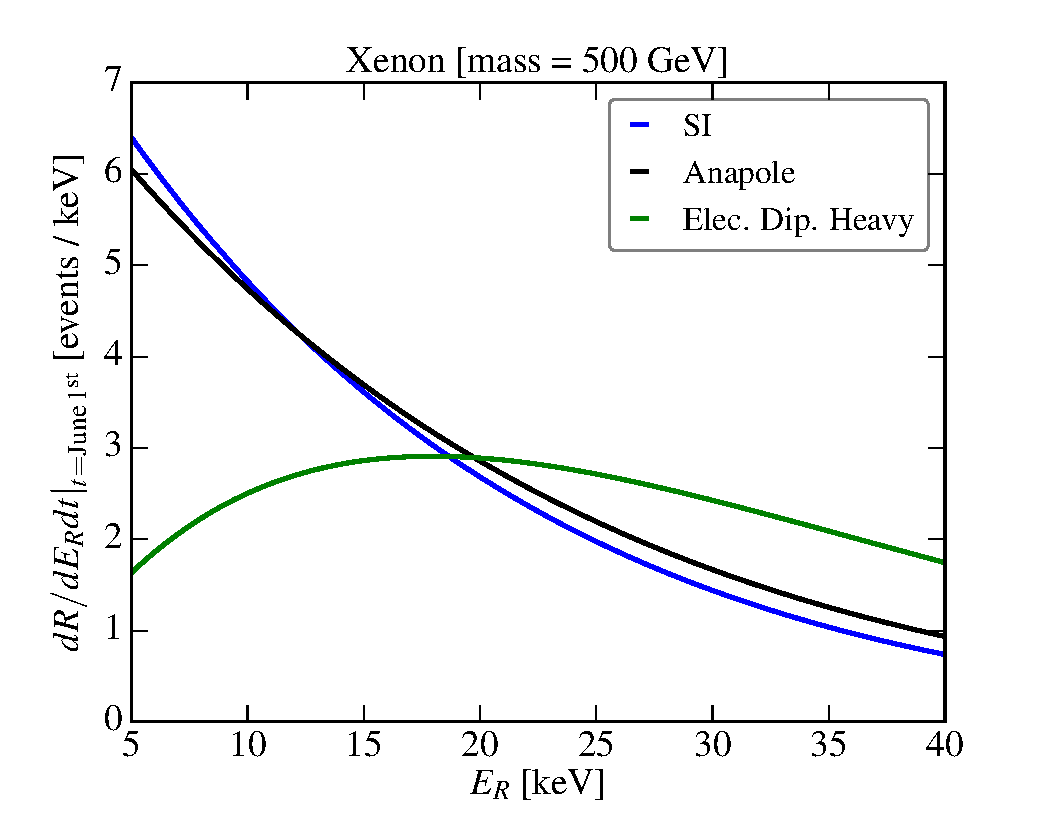
\includegraphics[width=0.49\textwidth, trim=0.cm 0.0cm 0.cm 0.0cm,clip=true]{plots/RecoilComparison_500GeV.pdf}
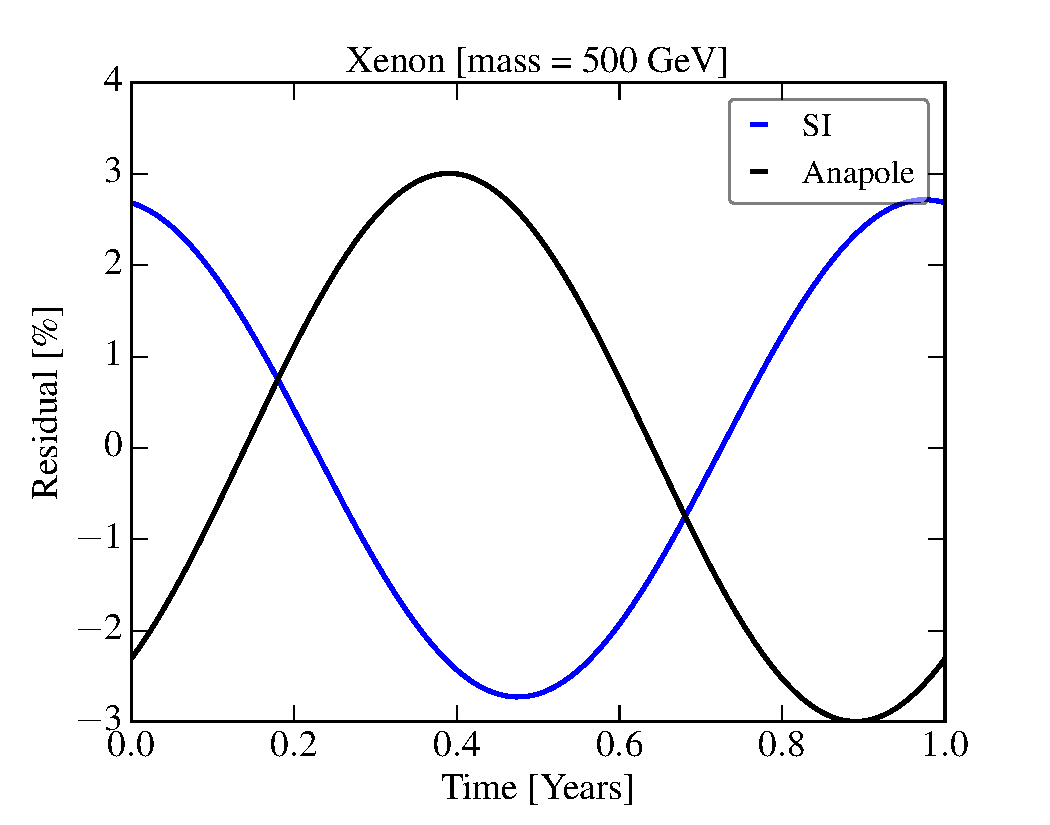
\includegraphics[width=0.49\textwidth, trim=0.cm 0.0cm 0.cm 0.0cm,clip=true]{plots/Xenon_SIvsAnapole_500GeV_Residual_Theory.pdf}
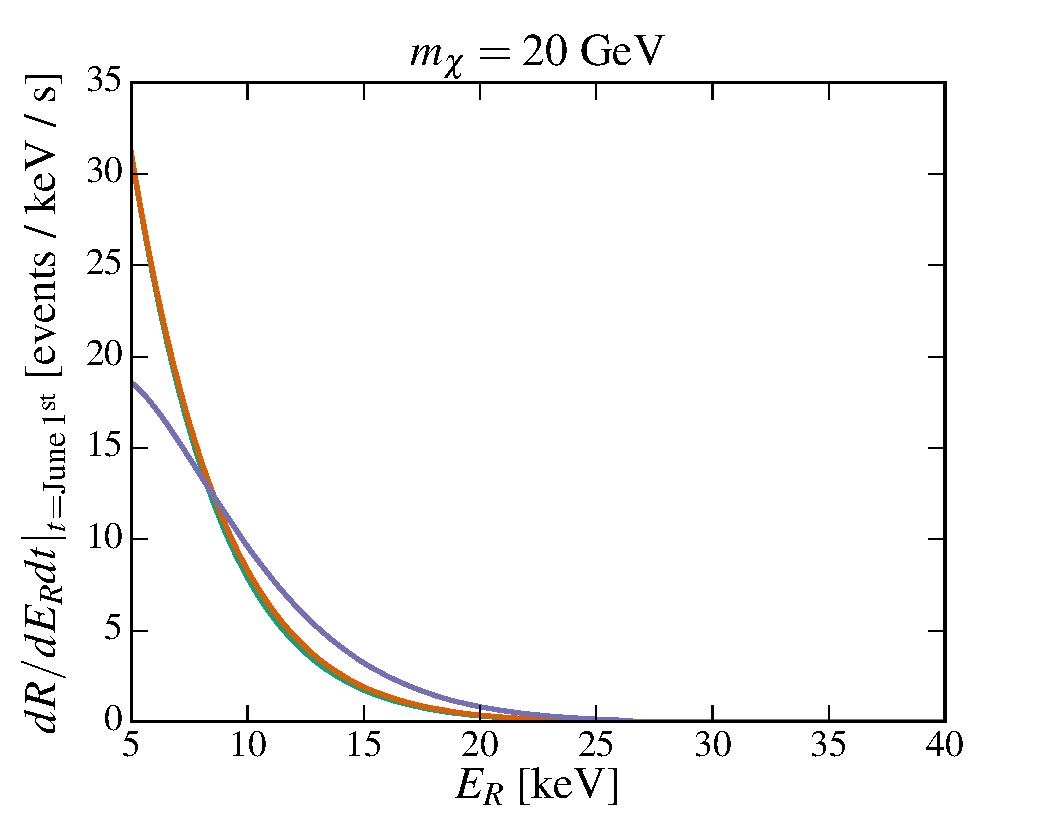
\includegraphics[width=0.49\textwidth, trim=0.cm 0.0cm 0.cm 0.0cm,clip=true]{plots/RecoilComparison_20GeV.pdf}
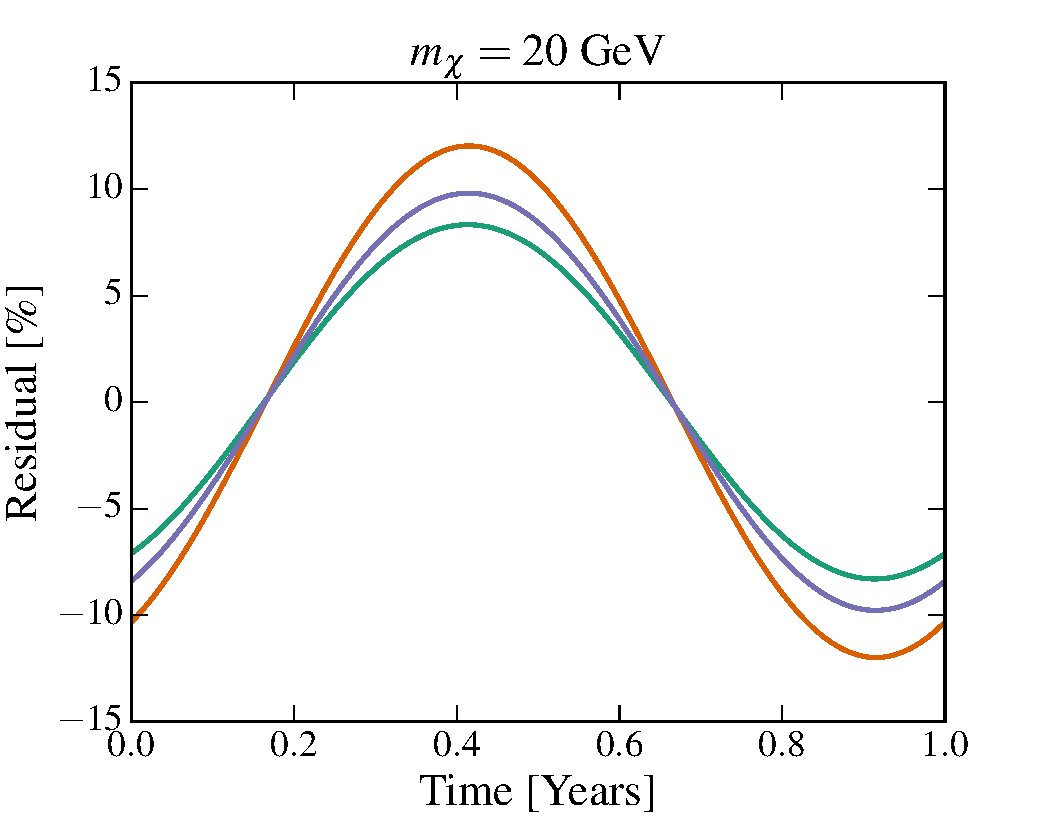
\includegraphics[width=0.49\textwidth, trim=0.cm 0.0cm 0.cm 0.0cm,clip=true]{plots/Xenon_SIvsAnapole_20GeV_Residual_Theory.pdf}
\caption{\label{fig:diff_rate_comp}
Comparing the energy (left) and time (right) dependence of the SI (blue), anapole (black), and ED-heavy (green) interactions in a xenon target. \emph{Left:} Differential rate evaluated at June $1^{st}$ as a function recoil energy for a $500$ GeV (top) and $20$ GeV (bottom) dark matter particle. \emph{Right:} Residual, defined to be the fractional deviation in the rate as a function of time (\ie $(\bar{R} - R(t))/\bar{R}$), for a $500$ GeV (top) and $20$ GeV (bottom) dark matter particle. Cross sections have been normalized to the current upper limit. }
\end{figure*}

The function $\sigma_T$ contains the interesting particle physics of the dark matter scattering and determines the energy and time dependence of the rate. In this section, \sjwrm{we discuss that this scattering can take only a limited number of forms which are catalogued by an effective field theory} \sjw{we summarize the effective theory that catalogues the basis-set of dark matter-nuclei interactions probed by direct detection experiments}. We highlight several particularly interesting examples of this scattering, \sjwrm{which we will subsequently use to test the effects of time dependence on model selection} \sjw{and subsequently use these models to quantify the extent to which including the time information of nuclear recoils can enhance model identification}.

\subsection{Momentum and Velocity Suppression: Scaling in Energy and Time}

Direct detection experiments consist of a low-background, radio-pure fiducial target consisting of a single element or molecule. The elements are chosen to have large principal quantum numbers, according to which the experiment falls into one of two categories: spin-independent or spin-dependent \sjwtt{Not sure I like this, I don't really see elements categorized this way -- these dichotomy is in my mind more what experiments feed funding agencies...  }. Spin-independent scattering involves coherent contributions from an entire nucleus, such that the cross section scales quadratically with nucleon number. This is to be contrasted with the spin-dependent rate\sjwrm{, since total nuclear spin is typically concentrated in a single nucleon and does not scale with nuclear size}\sjw{ which scales with the total nuclear spin, a quantity that is typically concentrated in a single nucleon}. Thus, experiments are often based on elements with large $A$ or large total spin, with the former experiments dubbed ``spin-independent'' and exhibiting reach to smaller absolute values of the overall cross section. \sjwtt{Again, not huge fan of this language. I would maybe prefer to emphasize the diversity in targets allows for a more generic probe of dark matter interactions}

Such reasoning obscures the fact that this classification strictly refers to the dependence on nuclear spin, and does not necessarily imply a hierarchy of expected rates. Many responses sensitive to a diversity of nuclear ``charges'' and ``currents'' can be classified as ``spin-independent'' \cite{Fitzpatrick:2012ix}, most of which are suppressed by small kinematic factors. Suppression of spin-independent scattering can lead to novel signatures in direct detection experiments. Consistently counting the pertinent small factors, and thus acquiring intuition for what might be seen in future experiments, requires a proper effective field theory expansion. The effective field theory of dark matter direct detection \cite{Fitzpatrick:2012ix, Anand:2013yka} is an expansion in two small kinematic variables: $|\vec q|/m_N$, where $\vec q$ is the change in momentum of the dark matter particle during the scattering, and $|\vec v_\perp|$, the (orthogonal component of the) relative velocity of the initial state particles. For an incoming (outgoing) dark matter three-momentum $\vec p(\vec p')$, incoming (outgoing) target three-momentum $\vec k(\vec k')$, and reduced mass $\mu_{\chi N} = m_\chi m_N/(m_\chi +m_N)$, we define these kinematic factors as \sjwtt{this is for elastic scattering} \cite{Fitzpatrick:2012ix}
\beq \label{eq:kinematic-definitions}
\vec q=\vec p'-\vec p=\vec k-\vec k', \qquad \vec v_\perp=\frac{\vec p}{m_\chi}-\frac{\vec k}{m_N}+\frac{\vec q}{2\mu_{\chi N}}.
\eeq
The momentum transfer is directly related to the nuclear recoil energy $E_R$ via $\vec{q}^2 =2m_TE_R$.

These expansion parameters are of the same order of magnitude, but they manifest differently in the observables of the scattering. In particular, responses that enter at higher order in $|\vec q|/m_N$ deliver a vanishing rate at both small and large momentum transfer, with a maximum rate at some intermediate recoil energy. On the other hand, higher order terms in $| \vec v_\perp|$ monotonically decrease with energy, qualitatively similar to standard scattering. The novelty of the responses with $| \vec v_\perp|$ dependence, therefore, is not easy to assess given a single energy spectrum. One solution is to leverage ``target complementarity'' by using a different nucleus with incommensurate nuclear charges \cite{Gluscevic:2015sqa}. We take a different approach here, starting from the observation that rates with a response proportional to $| \vec v_\perp|^2$ \sjwrm{include a nonstandard velocity integral in \Eq{eq:dRdEr_general}}  \sjw{produce differential cross sections with non-standard dark matter velocity dependencies}\sjwrm{, leading to a novel dependence on laboratory velocity (as well as the astrophysical parameters) in the differential rate }\cite{Fitzpatrick:2010br}. Because the laboratory velocity is changing with time, the different dependence on this velocity implicitly leads to a nonstandard time dependence for the interactions whose scattering cross sections include a factor of $|\vec v_\perp|^2$. \sjwtt{Not fanatic about this last sentence. Perhaps this is just my perception, but I don't see the lab velocity as the key feature. Yes, without Earth's rotation there is no time dependence, but a different velocity dependence is not guaranteed to produce a different time dependence (eg $d \sigma / d \ER \propto v^0$ and $v^2$). This is a more complicated effect than I think is suggested.} For large enough dark matter mass, this nonstandard time dependence can \sjwrm{provide the} \sjw{produce a nearly} \sjwtt{(not exactly opposite, closer to 5 months)} {\it opposite phase} compared to the standard rate! \sjw{Furthermore, differential cross sections which contain multiple non-negligible terms with different dependences on $|\vec v_\perp|^2$ can produce an annual modulation that is completely unique to each target element~\cite{DelNobile:2015tza,DelNobile:2015rmp}.} \sjwrm{Thus, a new observable can reveal the novelty of the responses with $|\vec v_\perp|$ dependence: we can use phase information from rates with nonstandard velocity integrals to distinguish these from the standard rates.} \sjw{Thus, by exploiting information on the time dependence of nuclear recoils, it may be possible to distinguish effectively field theory operators with different $|\vec v_\perp|$ dependences.  }




%Distinguishing between rates with different momentum dependence is easy to do even when limiting to energy spectrum information from a single detector target element \cite{Gluscevic:2015sqa}. However, extracting the particle physics from two rates with the same momentum dependence requires additional information. This is true because interactions with different momentum dependence have qualitatively different energy spectra, whereas those with the same momentum dependence (even if the $v_\perp$ dependence differs) have energy spectra whose differences may be hidden or suppressed by Poisson noise. The additional power needed for positive model selection can come from simultaneously examining spectra from detectors with complementary nuclear physics properties \cite{Gluscevic:2015sqa}. Alternately, a different route to this model discrimination may be provided by also analyzing the time information associated with the nuclear recoils.

As an example, we show in \Fig{fig:diff_rate_comp} how different momentum and velocity dependences alter the energy (left) and time (right) dependence of the SI, anapole, and heavy mediator electric dipole (ED-heavy) interactions, assuming a $500$ GeV (top) and $20$ GeV (bottom) dark matter particle. Instead of plotting the differential rate as a function of time in the right panel of \Fig{fig:diff_rate_comp}, we instead plot the residual, defined as the fractional deviation from the time-averaged energy integrated rate (\ie Residual $\equiv (\bar{R} - R(t))/\bar{R}$). The energy spectra for the SI and ED-heavy interactions are visually distinguishable in a way that the SI and anapole interactions are not: it does not take an arbitrarily large exposure to collect a sufficient number of events to distinguish between the SI and ED-heavy hypotheses using the energy spectrum alone, although doing the same with the SI and anapole hypotheses is quite challenging, given realistic Poisson errors \cite{Gluscevic:2015sqa}. However, as a function of time it is clear that the anapole and SI rates have different phases as functions of time. This difference, expected to be a few percent given standard calculations for the modulation power fraction, is not sufficiently powerful on its own to differentiate two models with similar energy spectra. Nonetheless, we will show below that this small effect can be leveraged to supplement the energy spectrum information, in turn allowing for successful model selection with a smaller number of total events than would be required using energy spectrum information alone.



\subsection{Summary of Models}

With this physics motivation in mind, we examine the ability to perform model selection on models of new physics with a heavy gauge boson of mass $M$ that kinetically mixes with the Standard Model photon. At high energies, the Lagrangian contains
\beq \label{eq:UV-model}
\cL \supset -  m_X \bar X_i X^j + i \bar X_i \slashed D_{ij} X^j  - \frac12 M^2 A'_\mu A'^\mu  - \frac14 F'_{\mu \nu} F'^{\mu \nu} - \frac\epsilon2 F'_{\mu \nu} F^{\mu \nu}
\eeq
for a family of fermions (or charged supermultiplet) $X$ with flavor index $i$ charged under a $U(1)'$ with vector boson $A'_\mu$ and gauge field strength $F'_{\mu \nu}$. At low energies, the dark matter couples to the Standard Model nucleon current \cite{Gresham:2014vja},
\beq \label{eq:current}
\cJ_\mu = \partial^\alpha F_{\alpha \mu} = e \sum_{n,p} \bar N \pL Q_N \frac{K_\mu}{2m_N} -\widetilde \mu_N \frac{i \sigma_{\mu \nu}q^\nu}{2m_N} \pR N,
\eeq 
where $Q_{p(n)}=1(0)$ are the nucleon charges in units of the electron charge $e$, $K_\mu/2 = (k_\mu + k'_\mu)/2$ is the average nucleon momentum, and $\tilde{\mu}_N = {\text{magnetic moment} \over \text{nuclear magneton}}$ is the dimensionless magnetic moment of the nucleon. At low energies, the model in \Eq{eq:UV-model} can give a dark matter particle that probes several interesting nuclear currents. The current measured in the experiment is determined how the charges and low-energy dynamics of the $X$ particle(s) give rise to a dark matter particle $\chi$, which has interaction Lagrangian $\cL \supset \frac1{M^2} \cO_\chi^\mu \cJ_\mu$ with the current in \Eq{eq:current} \sjwtt{The previous sentence is very confusing, can you reword this?}. If $\chi$ is electromagnetically neutral, the possible operators are \cite{Gresham:2014vja, Gluscevic:2015sqa}
\begin{eqnarray} \label{eq:photon-DM-ops}
\cO_{\rm \chi, Anapole}^\mu & = & g^{\rm Anapole}\bar \chi \gamma^\mu \gamma_5 \chi, \\
\cO_{\rm \chi, MD}^\mu & = & \frac{g^{\rm MD}}{\Lambda}\bar \chi i \sigma^{\mu \nu} q_\nu \chi ,\\
\cO_{\rm \chi, ED}^\mu & = & \frac{g^{\rm ED}}{\Lambda} \bar \chi i \sigma^{\mu \nu} \gamma_5 q_\nu \chi.
\end{eqnarray}
As stated above, the interaction operator for $\chi$ is determined by the dynamics of the $X$ fermion(s). The anapole current in \Eq{eq:photon-DM-ops} will arise if charged $X^\pm$ states condense to form a neutral Majorana state $\chi$ \cite{Bagnasco:1993st}. The dipole currents form if an electromagnetically neutral $X^0$ couples to an electromagnetically charged pair of partner $X^\pm$ particles (of appropriate spin) \cite{Weiner:2012gm}. The scale at which the charged $X$ states are integrated out is $\Lambda$.

The simplicity of the model building and the rich assortment of momentum and velocity dependence appears in the EFT responses illustrates how generic ``novel responses'' are. We list the EFT classification of these operators in \Tab{tab:operators}. (This is an abbreviated version of the more exhaustive table that appeared in \cite{Gluscevic:2015sqa}, using results of \cite{Gresham:2014vja, Gluscevic:2015sqa}.% For additional details of the implementation of the effective theory in the context of model selection, we refer to the discussion in \cite{Gluscevic:2015sqa}.
) In this work, we will focus on differentiating responses that have the same momentum scaling but different velocity dependence.



\begin{table}[tb]
\begin{centering}
\renewcommand{\arraystretch}{1.3}
\begin{tabular}{c |>{$}c<{$}| >{$}c<{$} >{$}c<{$} c } \hline
 Model name & {\rm Lagrangian} & \text{$\vec q$, $v$ Dependence} &  {\rm Response}  
\\ \hline 
 SI & \frac g{M^2}\bar \chi \chi \bar N N & 1 & M
\\ \hline 
 \multirow{2}{*}{Anapole} & \multirow{2}{*}{$\frac g{M^2}\bar{\chi} \gamma^\mu \gamma_5 \chi \, \cJ_\mu $} & v_\perp^2 & M \\  
 & & \vec{q}^2/m_N^2 & \Delta + \Sigma' 
\\ \hline
\multirow{2}{*}{\pbox{20cm}{Magnetic Dipole (Heavy)}} & \multirow{2}{*}{$\frac g{\Lambda M^2} \bar{\chi} \sigma^{\mu \nu} \chi  \, q_\nu \cJ_\mu $} & \frac{\vec q^{\,4}}{\Lambda^4}+ \frac{\vec{q}^2 v_\perp^2 }{\Lambda^2} & M \\
 & & \vec q^{\,4}/\Lambda^4 & \Delta + \Sigma' 
\\ \hline
Electric Dipole (Heavy) & \frac g{\Lambda M^2} \bar{\chi} \sigma^{\mu \nu} \gamma_5 \chi \, q_\nu \cJ_\mu  & \vec{q}^2 /\Lambda^2 & M 
\\ 
\hline 
\multirow{2}{*}{\pbox{20cm}{Magnetic Dipole (Light)}} & \multirow{2}{*}{$\frac g{\Lambda M^2} \bar{\chi} \sigma^{\mu \nu} \chi F_{\mu\nu} $} & 1+ \frac{v_\perp^2 m_N^2}{\vec{q}^2 } & M \\
  & & 1 & \Delta + \Sigma' 
 \\ \hline
 Electric Dipole (Light) & \frac g{\Lambda M^2} \bar{\chi} \sigma^{\mu \nu} \gamma_5 \chi F_{\mu\nu}  & m_N^2/\vec{q}^2 & M 
 \\ \hline 
\end{tabular}
\caption{Selection of operators along with their EFT dependences, adapted from \cite{Gluscevic:2015sqa}. The labels `Light' and `Heavy' in the dipole models denote the magnitude of the mediator mass relative to the characteristic momentum transfer. The nucleon electromagnetic current $\cJ_\mu$ is defined in \Eq{eq:current}; the transverse velocity $v_\perp$ and three--momentum transfer $\vec q$ are defined in terms of the collision momenta in \Eq{eq:kinematic-definitions}; and $\Lambda$ is a heavy mass or compositeness scale appearing in the dipole models. The parametric momentum and velocity dependences (third column) schematically multiply the adjacent EFT response (fourth column). }
\label{tab:operators} 
\end{centering}
\end{table}



\begin{table*}[t] 
\setlength{\extrarowheight}{3pt}
\setlength{\tabcolsep}{12pt}
\begin{center}
\begin{tabular}{c||m{3cm}|m{3cm}|m{3cm}}
Interaction /target & Xe & Ge & F\\
\hline\hline 
$m_\chi$ [GeV] & (20, 125, 500) & (20, 125, 500) & (20, 125, 500) \\
\hline\hline 
SI& (103, 99, 98) & (9, 4, 4)& (5, 1, 2)\\ \hline
%Millicharge& (103, 103, 102)& (834, 203, 189)& (334, 107, 103)\\
%SD flavor-univ.& (103, 97, 95)& (11, 4, 4)& (2318, 708, 725)\\
Anapole& (103, 97, 96)& (11, 5, 5)& (36, 3, 3)\\ \hline
Mag. dip. heavy& (103, 89, 87)& (3, 4, 5)& (4, 1, 1)\\ \hline
Mag. dip. light& (103, 101, 101)& (34, 14, 14)& (86, 16, 15)\\ \hline
Elec. dip. heavy& (103, 91, 88)& (4, 4, 4)& (1, 0, 0)\\ \hline
Elec. dip. light& (103, 102, 101)& (61, 15, 14)& (40, 12, 12)\\ \hline \hline
\end{tabular}
\end{center}
\caption{Predicted number of events in Gen2 experiments for various interactions with xenon, germanium, and fluorine targets, and assuming a dark matter mass of ($20$ GeV, $125$ GeV, and $500$ GeV). The predicted number of events are calculated using a cross section set to the current 90\% upper limit. Labels `light' and `heavy' denote the relative relation between the mediator mass and the characteristic scale of momentum transfer. }
\label{tab:pred_events}
\end{table*}


\section{Model Selection} \label{sec:procedure}

In the following, we apply Bayesian model selection to assess the extent to which analyzing the time dependence of nuclear recoils can improve the ability of future direct detection experiments to properly identify the true dark matter-nuclei interaction. 
   

\begin{table*}[tbp]
  \setlength{\extrarowheight}{3pt}
  \setlength{\tabcolsep}{10pt}
  \begin{center}
	\begin{tabular}{c|m{2.3cm}m{4.2cm}m{2.8cm}}  
	Label & A (Z) & Energy window [keVnr] & Exposure [kg-yr] \\
	\hline
	Xe & 131 (54) & 5-40 & 2000 \\
	Ge & 73 (32) & 0.3-100 & 100  \\
%	I & 127 (53) & 22.2-600 & 212 \\
	F &  19 (9) & 3-100 & 606 \\
%	Na & 23 (11) & 6.7-200 & 38 \\
%	Ar & 40 (18) & 25-200 & 3000 \\
%	He & 4 (2) & 3-100 & 300 \\

	\hline
	Xe(x3) & 131 (54) & 5-40 & 6000 \\
	Xe(x10) & 131 (54) & 5-40 & 20 000 \\
	XeG3 & 131 (54) & 5-40 & 40 000 \\
%	I+ & 127 (53) & 1-600 & 424 \\
%	F+ &  19 (9) & 3-100 & 1200 \\
	\end{tabular}
  \end{center}
\caption{Mock experiments considered in this work. The efficiency and the fiducialization of the target mass are included in the exposure. The first group of experiments is chosen such to be representative of the reach of Gen2 experiments for Xe, Ge, and F. The exposure for Xe and Ge is chosen to agree with the projected exclusion curves for LZ and SuperCDMS presented in Ref.~\cite{Cushman:2013zza}. The second group of experiments is used to quantitatively assess the impact of including the timing information of nuclear recoils, in the analysis of a single target experiment, as a function of the observed number of events. }
\label{tab:experiments}
\end{table*}

\subsection{Simulations \label{sec:sims}}

To simulate future datasets, we assume the dark matter-nuclei interaction is given by one of the models in the left column of Table~\ref{tab:pred_events}, and that the dark matter mass is either $20$ GeV, $125$ GeV, or $500$ GeV. We then optimistically assume that direct detection experiments are on the verge of of detecting dark matter, and set the cross section to be the value maximally allowed by LUX~\cite{Akerib:2016vxi}. The predicted number of events in various Gen2 experiments (see Table~\ref{tab:experiments}) using this cross section for each interaction and mass are shown in Table~\ref{tab:pred_events}. 

For each simulation, the observed number of events is obtained by randomly selecting from a Poisson distribution with a mean given by the predicted number of events. The recoil energy and time of each event is then obtained by applying a rejection sampling algorithm to the two-dimensional differential scattering rate. 

We perform our analysis on a variety of futuristic direct detection experiments. Our initial analysis focuses on the potential of Gen2 experiments to differentiate pairs of interactions with highly degenerate recoil spectra (\eg the SI and anapole interaction). Specifically we focus on xenon, germanium, and fluorine based experiments. Since fluorine experiments measure only the energy integrated rate, information on recoil energies of individual events are always neglected.  The exposure and energy window of these experiments are summarized in Table~\ref{tab:experiments}. Throughout our analysis we assume unit detection efficiency and zero background. In addition to the aforementioned, we also consider the potential reach of a Generation 3 (Gen3) xenon experiment, as well as various xenon experiments with exposures lying somewhere between Gen2 and Gen3 (the properties of which are summarized in Table~\ref{tab:experiments}).    

\begin{figure}
\centering
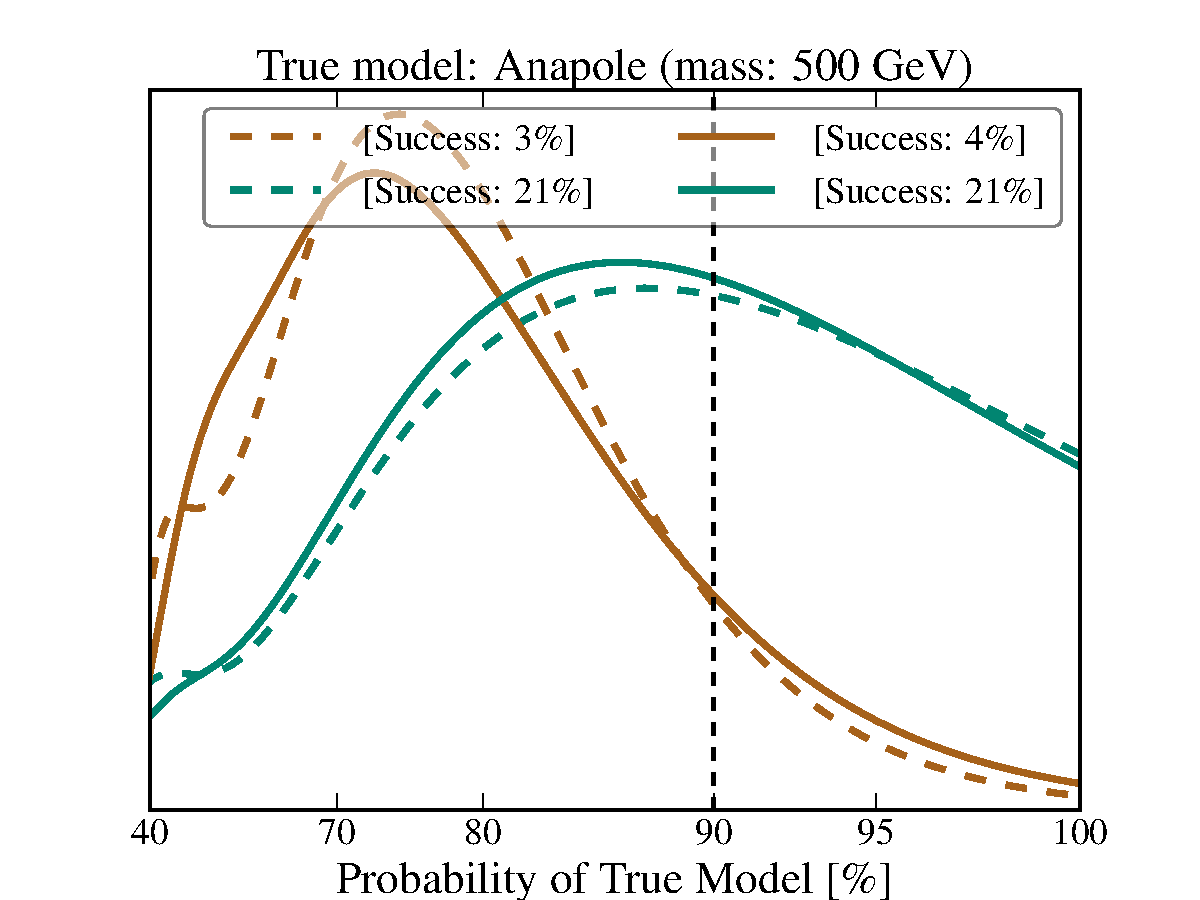
\includegraphics[width=0.45\textwidth]{plots/PDF_Single_500GeV_Anapole_50sims_Xe_vs_FGeXe_GF_TNT.pdf}
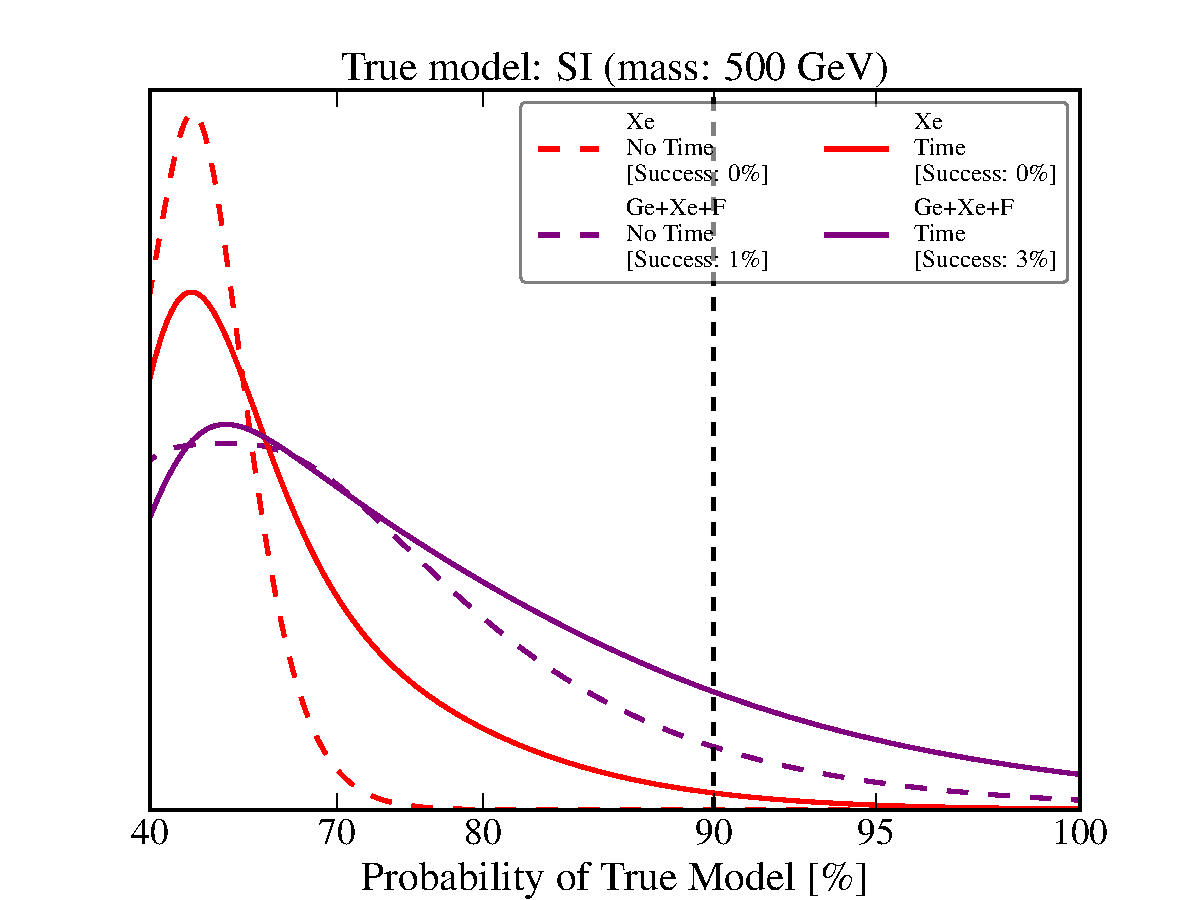
\includegraphics[width=0.45\textwidth]{plots/PDF_Single_500GeV_SI_Higgs_50sims_Xe_vs_FGeXe_GF_TNT.pdf}

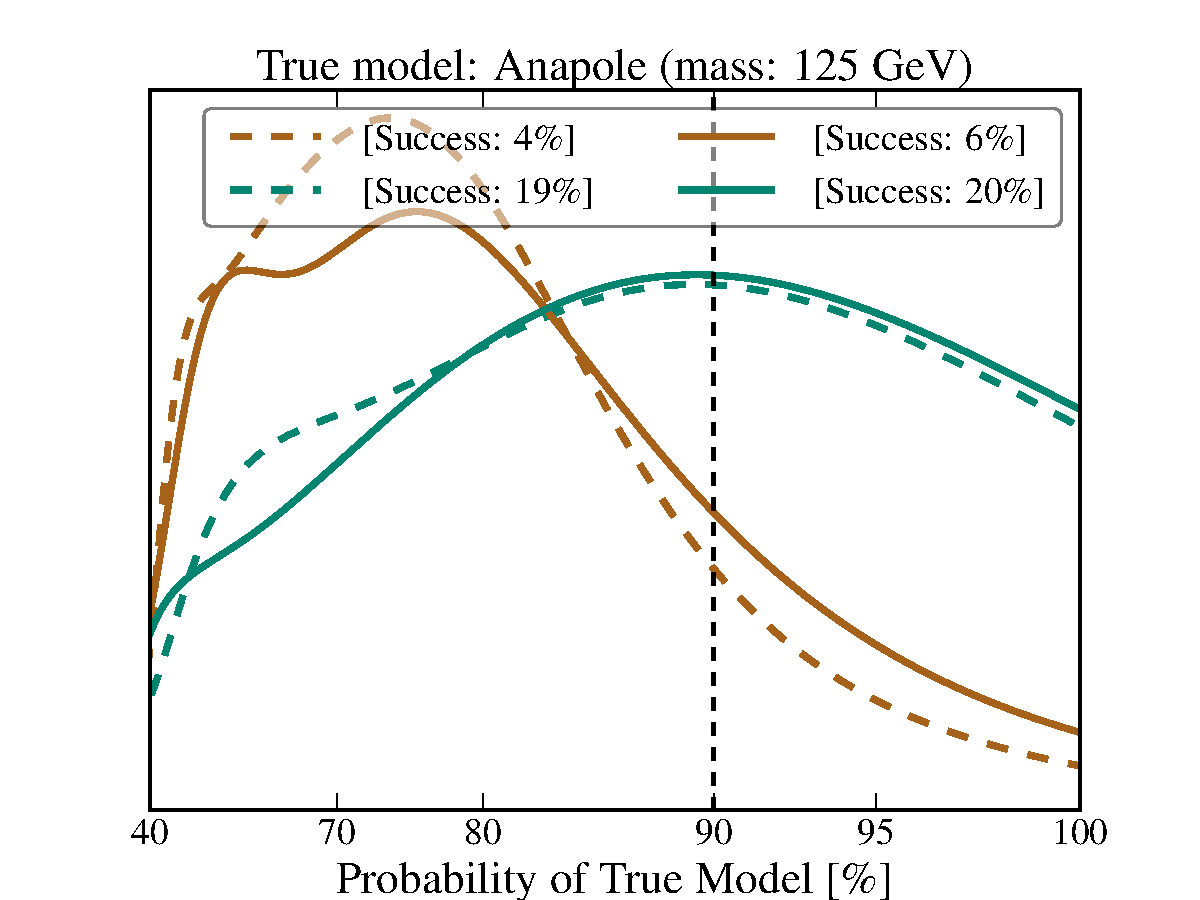
\includegraphics[width=0.45\textwidth]{plots/PDF_Single_125GeV_Anapole_50sims_Xe_vs_FGeXe_GF_TNT.pdf}
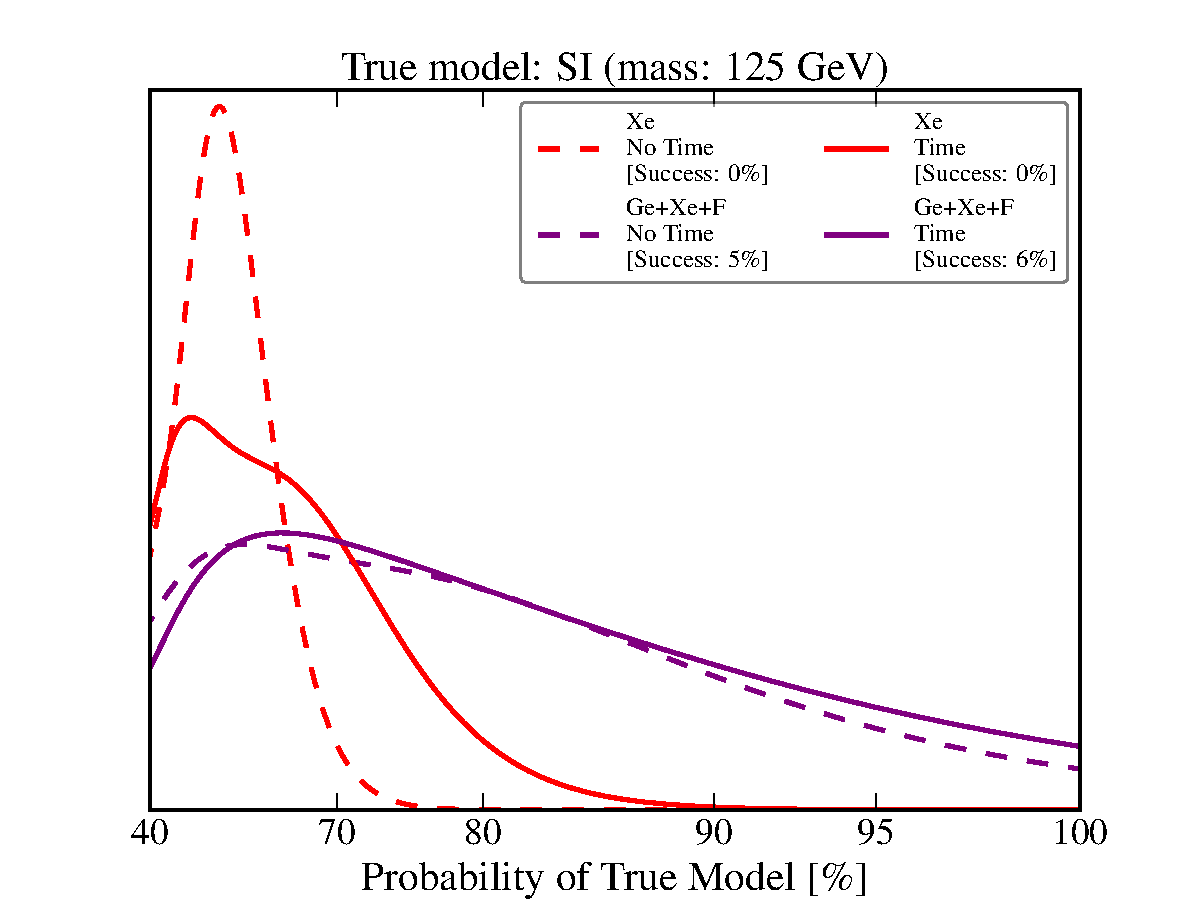
\includegraphics[width=0.45\textwidth]{plots/PDF_Single_125GeV_SI_Higgs_50sims_Xe_vs_FGeXe_GF_TNT.pdf}

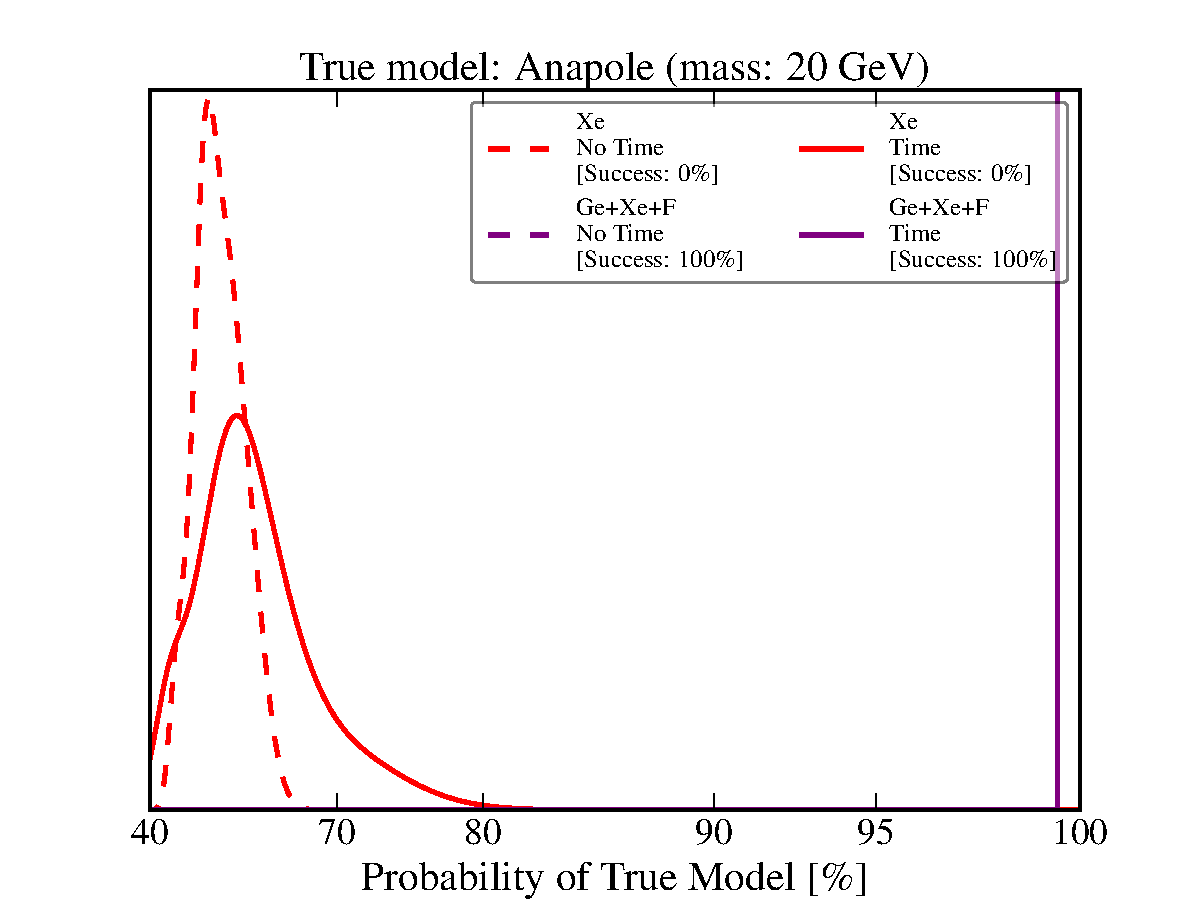
\includegraphics[width=0.45\textwidth]{plots/PDF_Single_20GeV_Anapole_50sims_Xe_vs_FGeXe_GF_TNT.pdf}
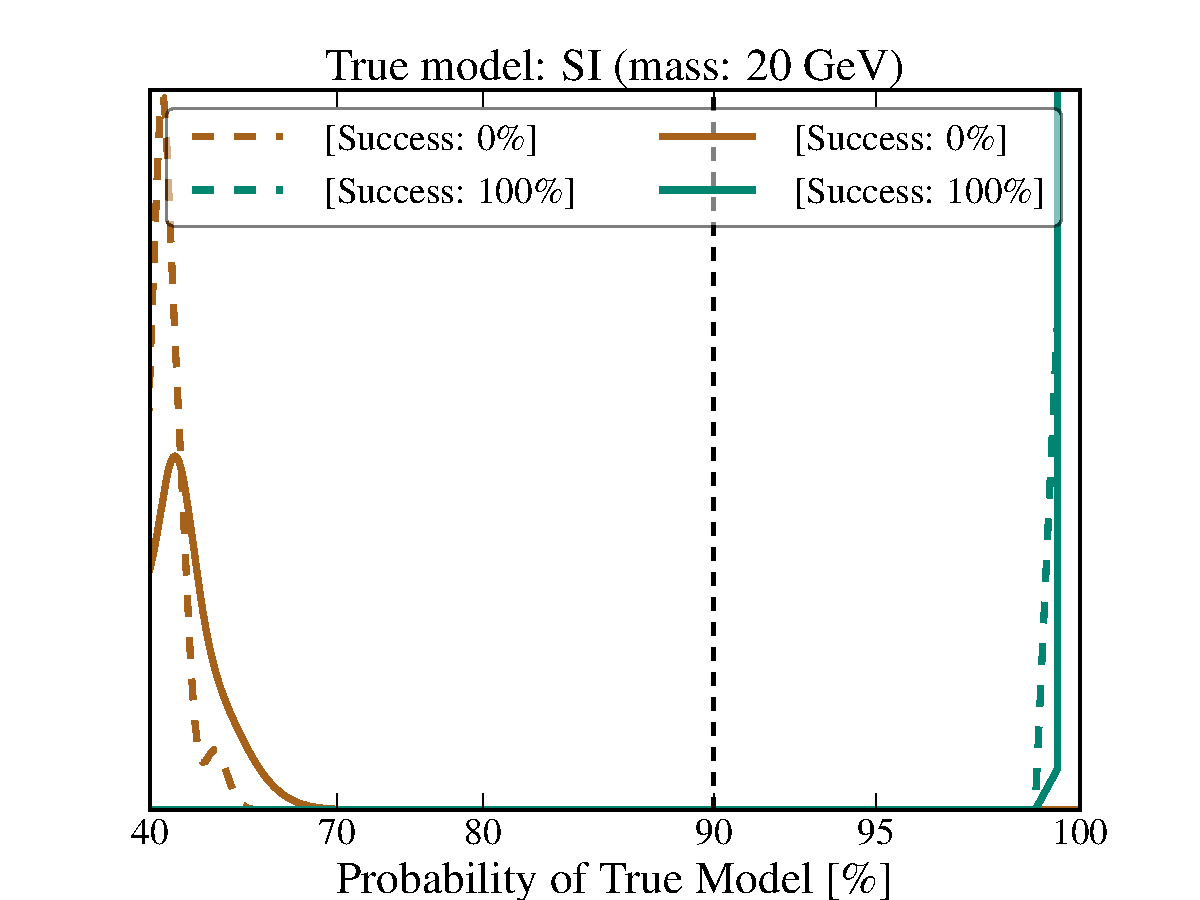
\includegraphics[width=0.45\textwidth]{plots/PDF_Single_20GeV_SI_Higgs_50sims_Xe_vs_FGeXe_GF_TNT.pdf}

\caption{\label{fig:gen2}
Model selection prospects with complimentary Gen2 targets. The normalized probability distribution functions for the probability of correctly identifying the true model are shown for the anapole (left) and SI (right) interactions, assuming a $500$ GeV (top), $125$ GeV (middle), and $20$ GeV (bottom) dark matter particle. Results are shown for a xenon experiment (red), and a combined analysis of xenon, germanium, and fluorine experiments (purple), including (solid) and neglecting (dashed) information on the modulation of the rate. Success rate is defined to be the fraction of realizations which produce correct model identification at the level of $ \geq 90\%$}
\end{figure}



\subsection{Data Analysis}

Within the Bayesian inference framework, the probability that the data $\vec{X}$ assigns to a given model $\cM_j$ is given by
\begin{equation}\label{eq:probs}
P(\cM_j) = \frac{\cE_j(\vec{X}|\cM_j)}{\sum_i \cE_i(\vec{X}|\cM_i)} \, ,
\end{equation}
where $\cE(\vec{X}|\cM)$ is the evidence of model $\cM$, defined by
\begin{equation}\label{eq:evidence}
\cE(\vec{X}|\cM) = \int d\Theta \, \cL(\vec{X}|\Theta,\cM) \, p(\Theta,\cM) \, ,
\end{equation}
and is intuitively understood to be the factor required to normalize the posterior $\cP$, \ie
\begin{equation}\label{eq:posterior}
\cP(\Theta | \vec{X}, \cM) = \frac{\cL(\vec{X}|\Theta,\cM)\, p(\Theta,\cM)}{\cE(\vec{X}|\cM)} \, . 
\end{equation}
Here, $\cL(\vec{X}|\Theta,\cM)$ is the likelihood, \ie the probability of obtaining the data, given a particular model $\cM$ and parameters $\Theta$ (for the purpose of this analysis $\Theta = \cbL m_\chi, \sigma_p \cbR$), and $p(\Theta, \cM)$ is the prior. In order to remain as agnostic as possible, we take wide priors in both $m_\chi$ and $\sigma_p$\footnote{Log priors are taken for both $m_\chi$ and $\sigma_p$, spanning $1-3000$ GeV in mass and $7$ orders of magnitude in cross section.}. In our analysis we use an unbinned extended likelihood function of the form
\begin{equation}\label{eq:likelihood}
\cL(\vec{X}|\Theta,\cM) = \frac{\mu^N}{N!} \, e^{-\mu} \, \prod_{x_i \in \vec{X}}\, \frac{1}{\mu} \, \frac{dR}{d\ER dt} \bigg|_{\ER,t \, = \, x_i} \, ,
\end{equation}
where $\mu$ is the predicted number of events, $N$ is the number of observed events, and the product runs over all the normalized differential rate evaluated at the $\ER$ and $t$ values of each observed event $x_i \equiv \cbL E_{R,i} \, , \, t_i \cbR$. When time or $\ER$ information is neglected, the differential rate is implicitly understood to be averaged over that variable. 

Our analysis proceeds as follows. We begin by simulating data for an experiment (or experiments) assuming a particular dark matter model, mass, and cross section (see Sec.~\ref{sec:sims}). We then use PyMultiNest to reconstruct the posterior defined in \Eq{eq:posterior}, and subsequently calculate the evidence for various dark matter models~\cite{pymultinest,Feroz:2008xx}\footnote{Multinest runs are performed with 2000 live points, an evidence tolerance of 0.1, and a sampling efficiency of 0.3.}. Once the evidence of various models has been computed, one can estimate the probability of successfully being able to identify the true model using \Eq{eq:probs}. This procedure is then repeated for $\simeq \cO(50)$ simulations to assess the variability in successful model identification arising from Poisson fluctuations. A model is said to be correctly identified if the probability determined using \Eq{eq:probs} is large. For the purpose of this paper, we define the boundary for successful model identification at $P \geq 90\%$. The primary quantity of interest for future direct detection experiments is then the fraction of simulations which lead to a successful model identification.    



Instead of plotting the individual probabilities of each simulation, we apply kernel density estimation (KDE) with a Gaussian kernel to determine the distribution functions of these probabilities. For of the results listed in the following section, we plot the KDE distribution for each experimental combination both with and without time, and determine the fractional success rate by integrating the distribution above the 90\% threshold. 


\begin{figure*}
\centering
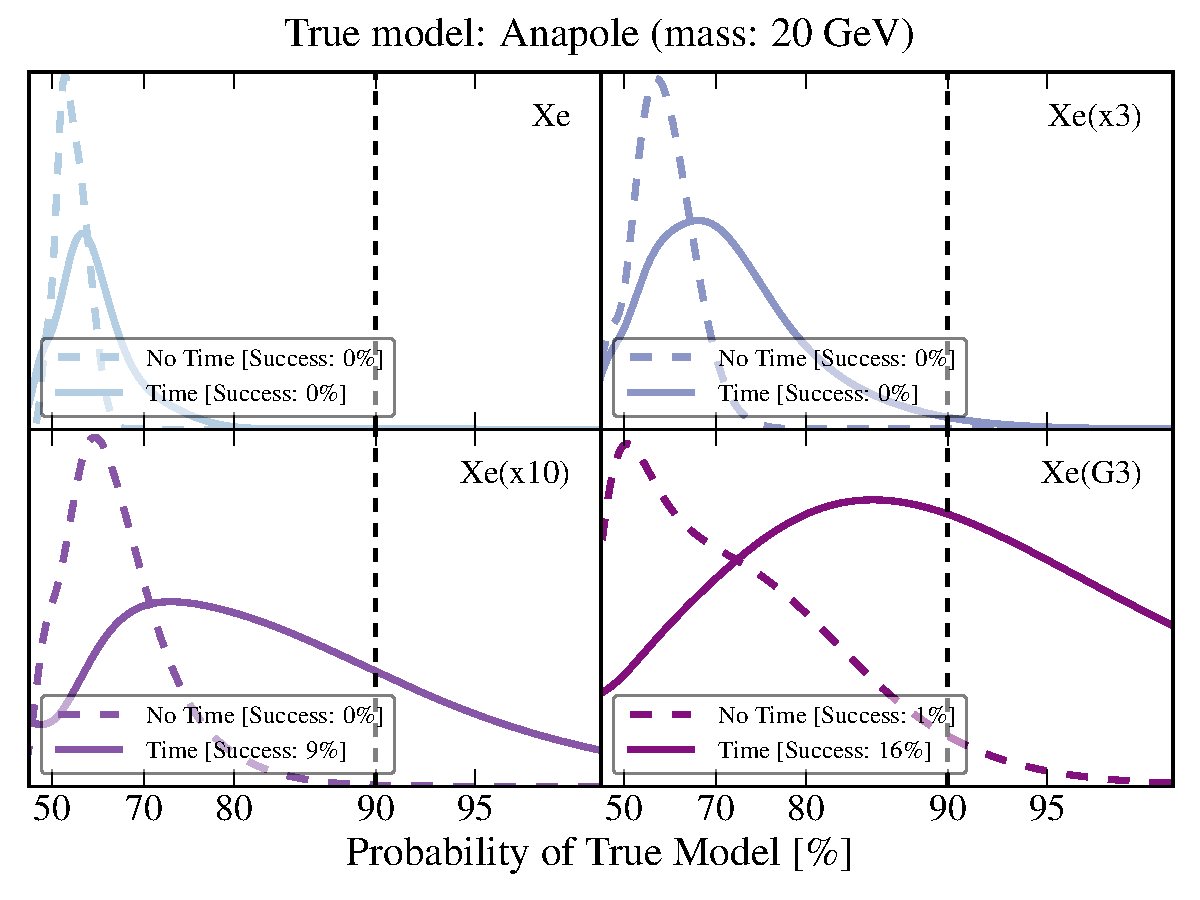
\includegraphics[width=0.7\textwidth]{plots/PDF_20GeV_Anapole_50sims_Xe_Xe3x_Xe10x_XeG3_GF_TNT.pdf}
\caption{\label{fig:20gev_anapole_XeFull_TNT_GF}
Model selection prospects for a single target (xenon), including (solid) and neglecting (dashed) information on the modulation of the rate. The normalized probability distribution functions are plotted for the probability associated with correcting identifying a 20 GeV dark matter particle scattering through the anapole interaction. Panels from left to right, top to bottom, correspond to exposure of 2 ton-years (blue), 6 ton-years (red), 20 ton-years (green), and 40 ton-years (magenta). Calculations are performed assuming the true cross section is sitting at the current $90\%$ upper limit. Successful model identification, defined as having $\geq 90 \%$ probability, are provided in the legend of each analysis.}
\end{figure*}



\section{Results}\label{sec:results}
We begin by considering the extent to which including time information in the analysis of Gen2 experiments can assist in breaking degeneracy between the SI and anapole interactions. Specifically, in \Fig{fig:gen2} we consider the probability of correctly identifying the anapole (left) and SI (right) interactions, assuming a putative signal is detected in either a xenon experiment (red) or in a combination of xenon, germanium, and fluorine experiments (purple). Analysis is shown for a $500$ GeV dark matter particle (top), $125$ GeV dark matter particle (middle), and a $20$ GeV dark matter particle (bottom), including (solid) and neglecting (dashed) information on the modulation. 

Consistent with the results of~\cite{Gluscevic:2015sqa}, we find that both models can be correctly identified in Gen2 experiments for a $20$ GeV dark matter particle, but only if detections are made in both xenon and fluorine based experiments (note that Xe+Ge analyses do not break the degeneracy and have no model discrimination). Should detections be made in both xenon and fluorine experiments, time information would not be needed to differentiate the two models.  



Correct model identification is slightly more complicated for heavier dark matter candidates due to the reduced scattering rate in fluorine. For the anapole model, detection in Xe leads to a model discrimination of a few percent. If however, detections are made in xenon, germanium, and fluorine experiments, model selection could be as high as $\simeq 20 \%$. Including time information only increases model selection by $\cO(1)\%$ in both cases. Model selection for the SI interaction is significantly reduced relative to that of the anapole interaction. Xenon experiments are completely unable to break this degeneracy if massive dark matter interacts through a SI interaction, regardless of whether or not time information is included in the analysis. Should detections be made in xenon, germanium, and fluorine experiments, correct model identification is still only at the level of a few percent. As with the anapole interaction, including time information in the analysis has the potential to improve model selection by $\cO(1)\%$. 

\begin{figure*}
\centering
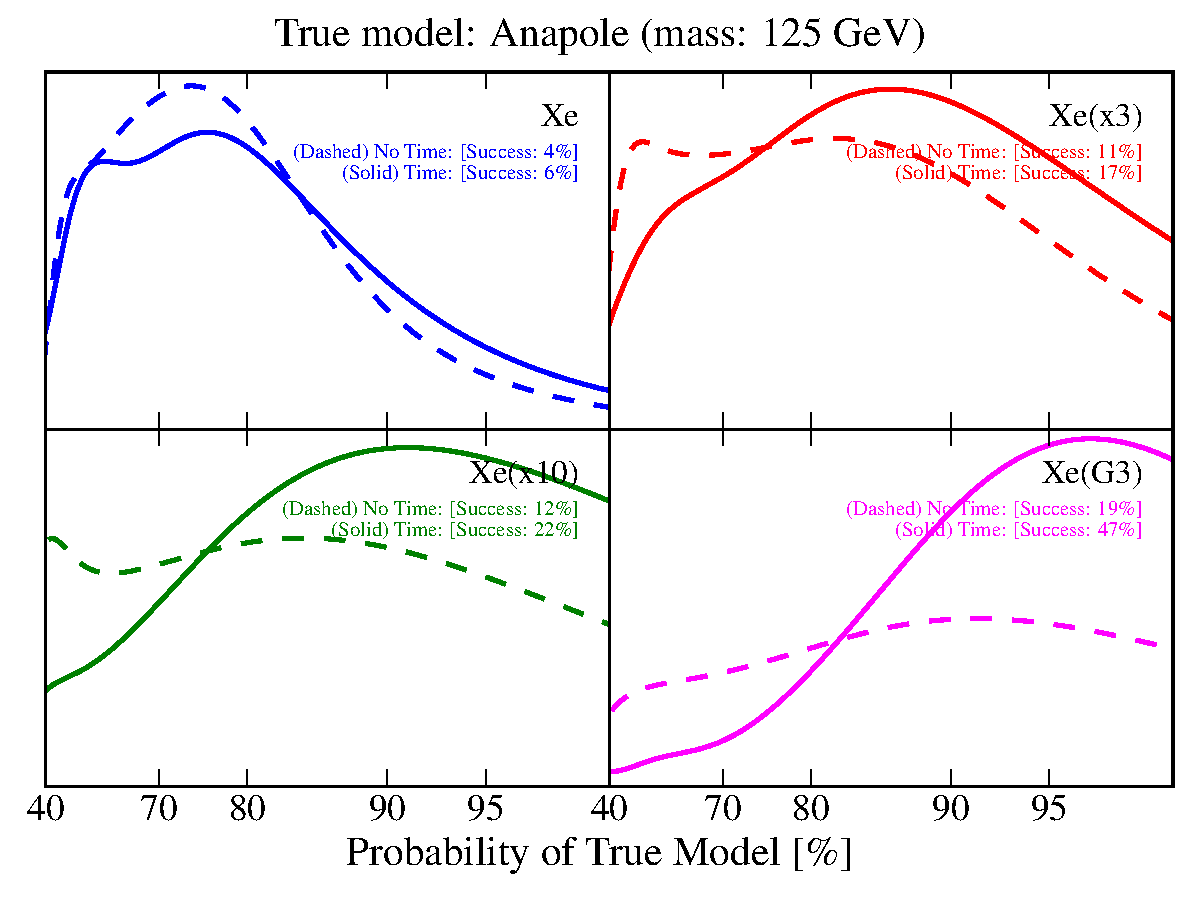
\includegraphics[width=0.7\textwidth]{plots/PDF_125GeV_Anapole_50sims_Xe_Xe3x_Xe10x_XeG3_GF_TNT.pdf}
\caption{\label{fig:125gev_anapole_XeFull_TNT_GF}
Same as Fig.~\ref{fig:20gev_anapole_XeFull_TNT_GF} but for $125$ GeV dark matter.}
\end{figure*}

Given that Gen2 experiments will optimistically detect $\simeq 100$ events for the SI and anapole interaction, it is not surprising that analyzing Gen2 data with time has a minimal effect on model selection (see \eg Sec.~4 of \cite{DelNobile:2015nua} for an estimation of the number of events needed for phase discrimination). Perhaps the more interesting question is: how many events are needed before the inclusion of time information can significantly effect model selection? We address this question in the context of the breaking the SI and anapole degeneracy in xenon based experiments in Figs.~\ref{fig:20gev_anapole_XeFull_TNT_GF}-\ref{fig:500gev_anapole_XeFull_TNT_GF}. For 20, 125, and 500 GeV anapole dark matter, we plot the probability of correctly identifying the true model in a 2 ton-year (blue), 6 ton-year (red), 20 ton-year (green), and 40 ton-year (magenta) xenon experiment, neglecting (dashed) and including (solid) time information. Since results for the SI interaction are qualitatively similar to that of the anapole, we defer the SI analogues of Figs.~\ref{fig:20gev_anapole_XeFull_TNT_GF}-\ref{fig:500gev_anapole_XeFull_TNT_GF} to Appendix A. 

\Fig{fig:diff_rate_comp} clearly shows that the recoil spectrum observed in xenon arising from light anapole and SI dark matter is more degenerate than that of heavy anapole and SI dark matter. Unfortunately the phase of light dark matter is also degenerate for conventional velocity dependent cross sections (\ie $d\sigma/d\ER \propto v^{-2}, v^0, v^2, ...$)~\cite{DelNobile:2015tza,DelNobile:2015rmp}, suggesting that the inclusion of time information in the analysis may not be sufficient to fully differentiate these models. Indeed \Fig{fig:20gev_anapole_XeFull_TNT_GF} shows that even in a Gen3 xenon experiment, the SI and anapole interaction can only be correctly identified in $\simeq 15\%$ of our simulations (assuming time is included). Perhaps surprisingly, however, is that the inclusion of time in the analysis improves model discrimination by $\simeq 15\%$. This improvement arises not from differences in the phase, but rather from the amplitude of the modulation, which as shown in \Fig{fig:diff_rate_comp} differs by $\simeq 5\%$.



As the dark matter mass increases the recoil spectrum become less degenerate, allowing for better model discrimination at fixed exposure. Additionally, heavier dark matter allows these experiments to probe regions of parameter space where the anapole and SI interaction are out of phase (see \Fig{fig:diff_rate_comp}). Figs.~\ref{fig:125gev_anapole_XeFull_TNT_GF} and \ref{fig:500gev_anapole_XeFull_TNT_GF} confirm that heavier dark matter candidates allow for better model discrimination of these models, particularly when time is included in the analysis. We emphasize that including time in the analysis can potentially improve model selection in Gen3 experiments by as much as $\simeq 30\%$ for heavy dark matter candidates, where the phase of these interactions may be misaligned by as much as $\simeq 5$ months. Despite this improvement, Gen3 experiments will likely also need to exploit target complimentarily to in order to fully break the SI-anapole degeneracy. 

To briefly summarize the conclusions of Figs.~\ref{fig:20gev_anapole_XeFull_TNT_GF}-\ref{fig:500gev_anapole_XeFull_TNT_GF}, including time information in the analysis of future xenon direct detection experiments begins to significantly enhance model selection after $\simeq \cO(1000)$ ($ \cO(300)$) events have been observed, assuming a 20 (500) GeV dark matter particle. Gen3 xenon experiments can perhaps expect an enhancement in model selection as large as $30\%$ (for the SI this enhancement can be as large as $\simeq 40\%$) for the most optimistic of circumstances, but will still require target complementarity to definitely identify the correct model.  

\begin{figure*}
\centering
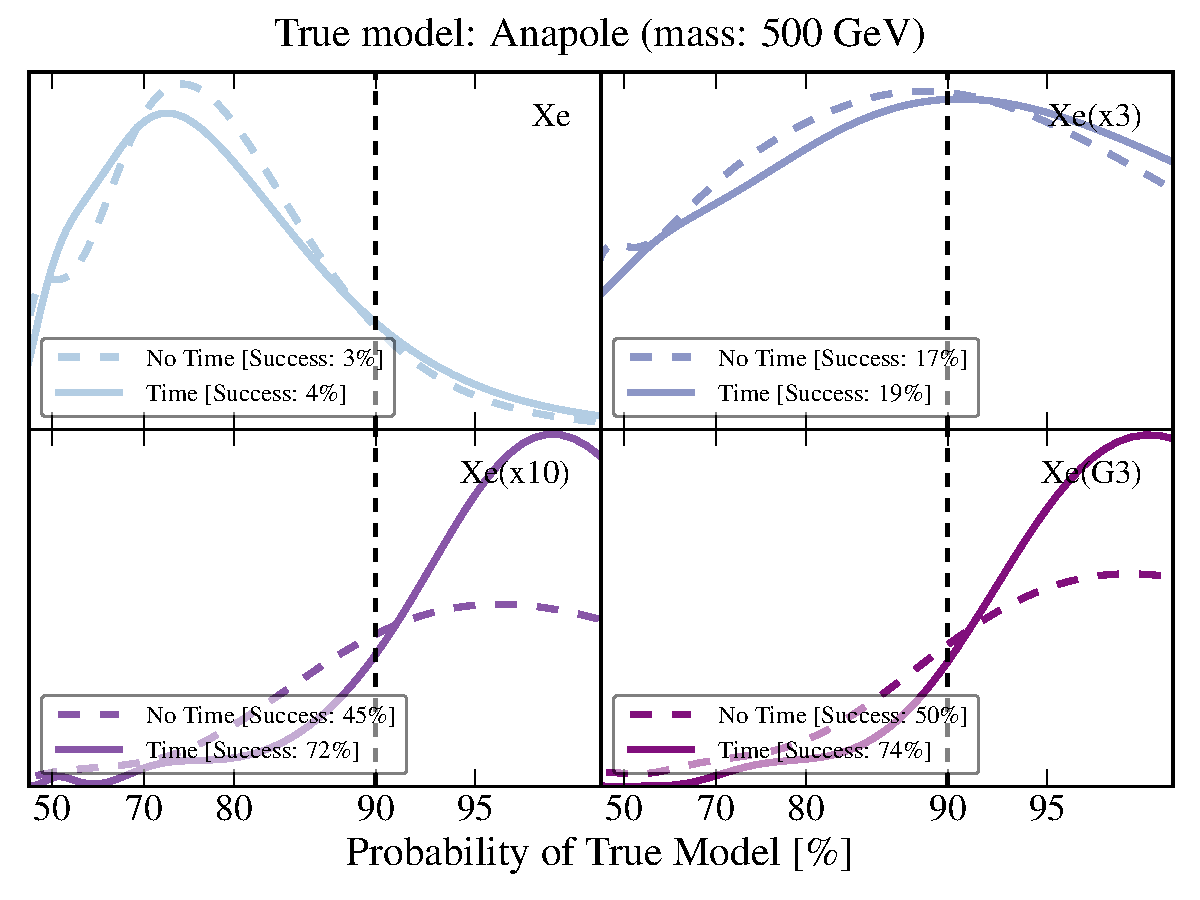
\includegraphics[width=0.7\textwidth]{plots/PDF_500GeV_Anapole_50sims_Xe_Xe3x_Xe10x_XeG3_GF_TNT.pdf}
\caption{\label{fig:500gev_anapole_XeFull_TNT_GF}
Same as Fig.~\ref{fig:20gev_anapole_XeFull_TNT_GF} but for $500$ GeV dark matter.}
\end{figure*}

We would like to emphasize that the purpose of this paper is not of a comparison of the SI and anapole interactions, but rather a quantitative assessment of whether time information can be exploited in future direct detection analyses to break degeneracies in the recoil spectrum. The SI and anapole interactions provide one particularly illuminating example of this because they contain different dependencies on the dark matter velocity (and consequently have a different modulation). Despite also having an approximately degenerate recoil spectrum in xenon, the same cannot be said for the SI and SD interactions which have the same dark matter velocity dependence. There do exist, however, other illustrative examples which we briefly consider below.

In \Figs{fig:125gev_Mag.dip.heavy_XeFull_TNT_GF}{fig:125gev_Mag.dip.light_XeFull_TNT_GF} we consider a comparison of the magnetic dipole and electric dipole interactions for a $125$ GeV dark matter particle, assuming a heavy (\Fig{fig:125gev_Mag.dip.heavy_XeFull_TNT_GF}) and light (\Fig{fig:125gev_Mag.dip.light_XeFull_TNT_GF}) mediator. As before we consider putative detections in future xenon experiments with exposures varying from 2 ton-years to 40 ton-years. The results are rather similar to the SI and anapole comparison in that Gen3 experiments can expect a $\simeq 20\%$ improvement in model selection when time is included in the analysis, but again necessitate target complementarity to fully differentiate these models.








\section{Conclusions}\label{sec:conclusion}
We have considered here the potential impact of using time information in the analysis of future direct detection experiments to break approximate degeneracies that may appear between the recoil spectrum of different interactions. Specifically, we have applied Bayesian model selection to simulated data sets that include the impact of Poisson fluctuations to quantitively assess future ability of xenon experiments to successfully identify approximately degenerate models, assuming analyses include and neglect the time information of detected recoils.

 
 \begin{figure*}
\centering
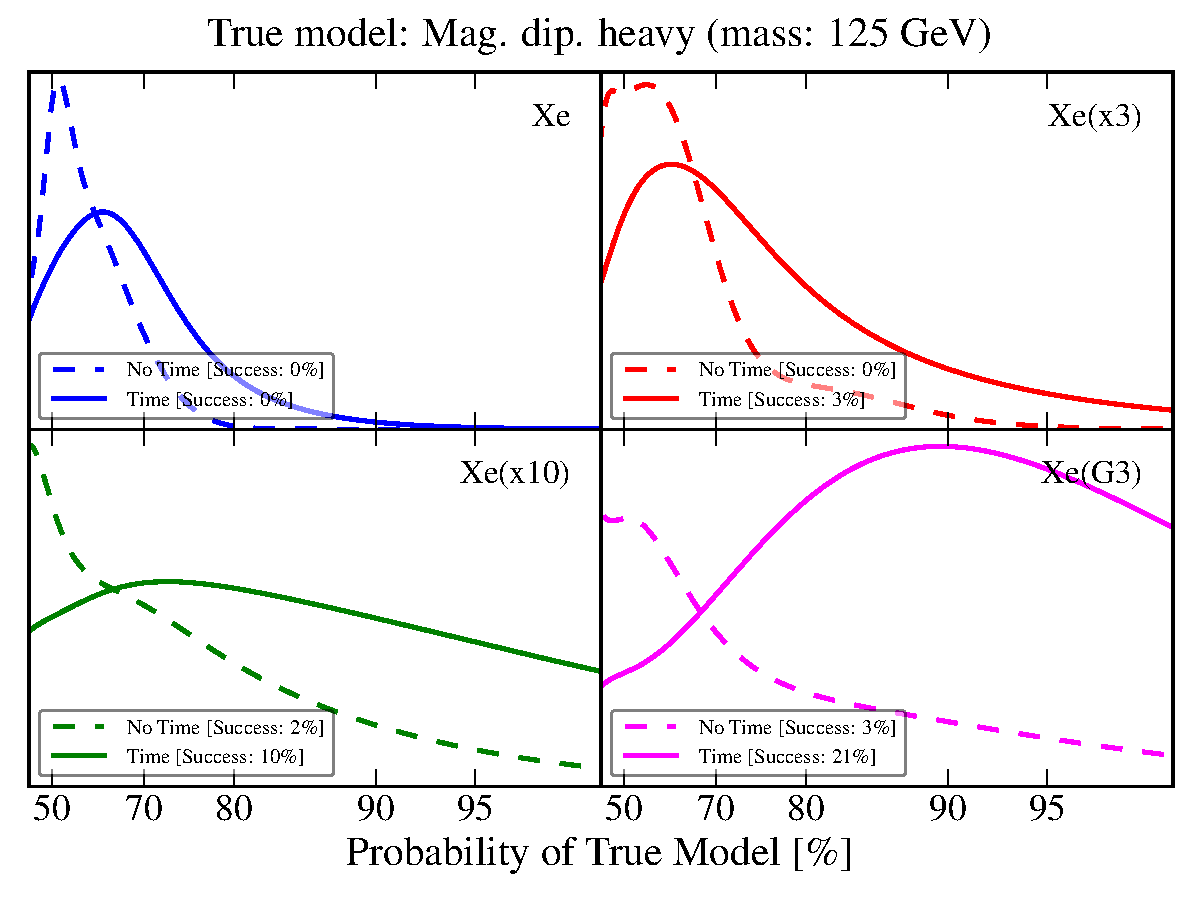
\includegraphics[width=0.7\textwidth]{plots/PDF_125GeV_Magdipheavy_50sims_Xe_Xe3x_Xe10x_XeG3_GF_TNT.pdf}
\caption{\label{fig:125gev_Mag.dip.heavy_XeFull_TNT_GF}
Same as Fig.~\ref{fig:20gev_anapole_XeFull_TNT_GF}, but now assessing the ability of xenon experiments to break the degeneracy of the magnetic dipole (heavy mediator) and electric dipole (heavy mediator). Results are shown for a $125$ GeV dark matter and and assuming the magnetic dipole is the true model.}
\end{figure*}


In a comparison of the SI and anapole interactions, we have found that under the most optimistic of circumstances Gen2 direct detection experiments can only expect an increase in model selection of $\simeq \cO(1)\%$ when time is included in the analysis, and only if target complementarity is simultaneously exploited. We have shown that a significant ($\simeq \cO(10)\%$) increase in model selection between these two interactions requires $\simeq \cO(1000)$ ($\cO(300)$) events to be observed in xenon detector, assuming a 20 (500) GeV dark matter particle. Furthermore, even if time is exploited in Gen3 xenon experiments, target complementarity must also be exploited to unequivocally differentiate these two models.

In addition to the aforementioned example, we have also provided an illustration of this analysis for a comparison of the magnetic dipole and electric dipole interactions. Quantitatively these results are quite similar to those of the SI and anapole interactions.

In the event of a putative signal, future direct detection experiments will be charged with the difficult task of illuminating the high energy behavior of dark matter solely from the observed low energy recoils. This is a particular daunting task in light of the fact that many feasible dark matter models produce nearly degenerate recoil spectra. Exploiting all of the information available, including the time information of nuclear recoils and detections in multiple experiments, will likely be required to make definitive statements regarding the true nature of dark matter.

\begin{figure*}
\centering
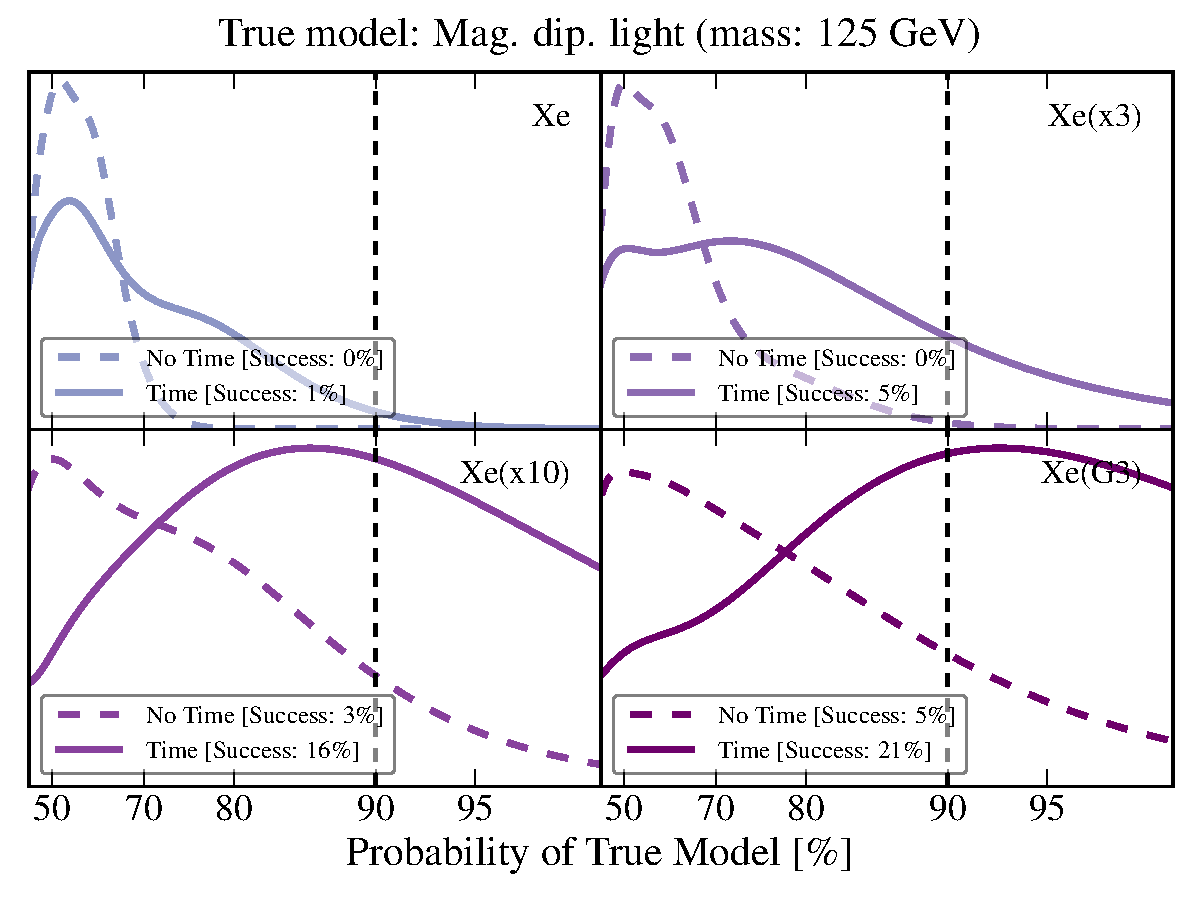
\includegraphics[width=0.7\textwidth]{plots/PDF_125GeV_Magdiplight_50sims_Xe_Xe3x_Xe10x_XeG3_GF_TNT.pdf}
\caption{\label{fig:125gev_Mag.dip.light_XeFull_TNT_GF}
Same as \Fig{fig:125gev_Mag.dip.heavy_XeFull_TNT_GF} but for a light mediator. }
\end{figure*}


\bigskip

\textbf{Acknowledgments.} SW is supported under the University Research Association (URA) Visiting Scholars Award Program, and by a UCLA Dissertation Year Fellowship. %Fermilab is operated by Fermi Research Alliance, LLC, under Contract No. DE-AC02-07CH11359 with the US Department of Energy. 

\appendix

\section{Model Selection Prospects in Xenon (SI Interaction)}
We present in Figs.~\ref{fig:20gev_SI_Higgs_XeFull_TNT_GF}-\ref{fig:500gev_SI_Higgs_XeFull_TNT_GF} the model selection prospects for various exposure xenon experiments, including (solid) and neglecting (dashed) information on the modulation of the rate, and assuming the SI interaction is the true model. Results are shown for $20$ GeV (\Fig{fig:20gev_SI_Higgs_XeFull_TNT_GF}), $125$ GeV (\Fig{fig:125gev_SI_Higgs_XeFull_TNT_GF}), and $500$ GeV (\Fig{fig:500gev_SI_Higgs_XeFull_TNT_GF}) dark matter. Results are similar to those presented in \Sec{sec:results} for the anapole interaction. 


\begin{figure*}
\centering
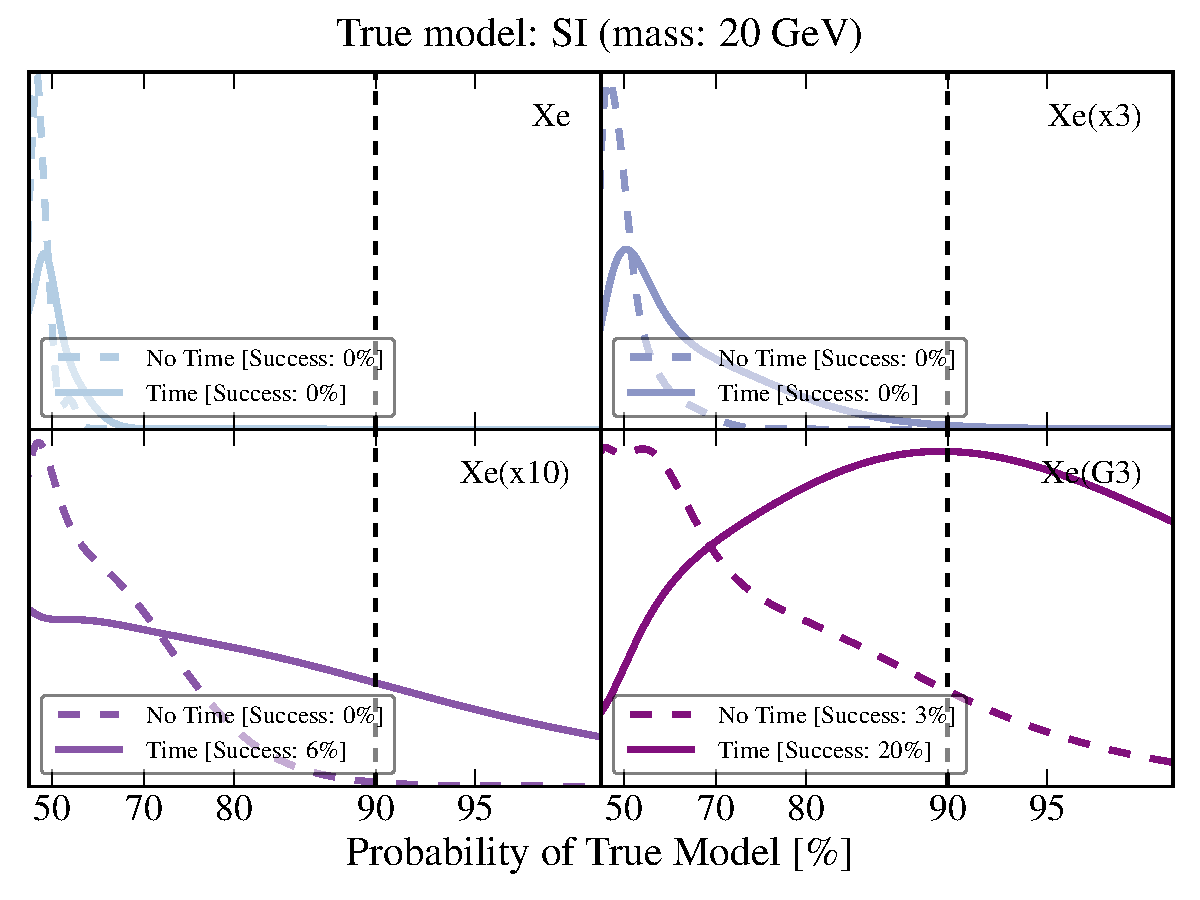
\includegraphics[width=0.7\textwidth]{plots/PDF_20GeV_SI_Higgs_50sims_Xe_Xe3x_Xe10x_XeG3_GF_TNT.pdf}
\caption{\label{fig:20gev_SI_Higgs_XeFull_TNT_GF}
Same as Fig.~\ref{fig:20gev_anapole_XeFull_TNT_GF} but for the SI interaction.}
\end{figure*}


\begin{figure*}
\centering
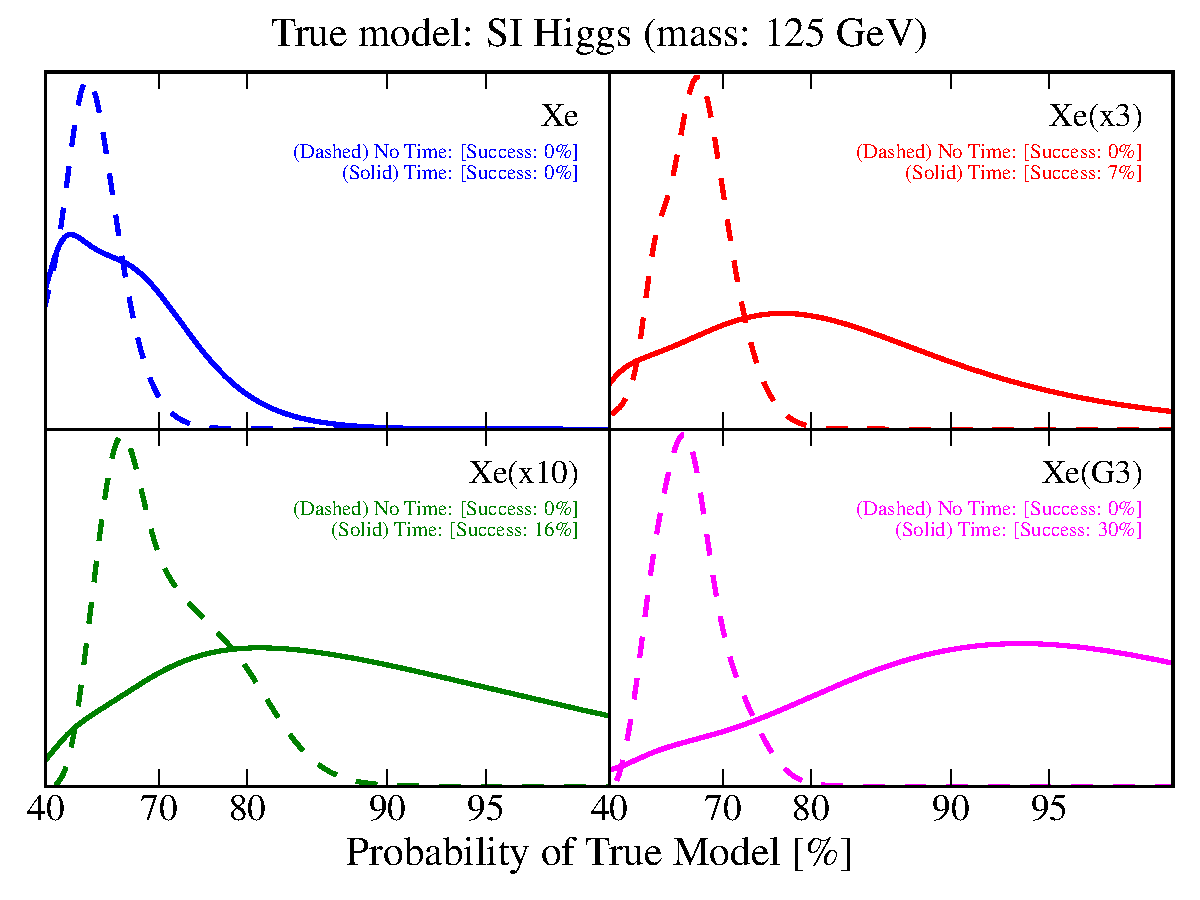
\includegraphics[width=0.7\textwidth]{plots/PDF_125GeV_SI_Higgs_50sims_Xe_Xe3x_Xe10x_XeG3_GF_TNT.pdf}
\caption{\label{fig:125gev_SI_Higgs_XeFull_TNT_GF}
Same as Fig.~\ref{fig:20gev_anapole_XeFull_TNT_GF} but for a $125$ GeV dark matter and the SI interaction.}
\end{figure*}


\begin{figure*}
\centering
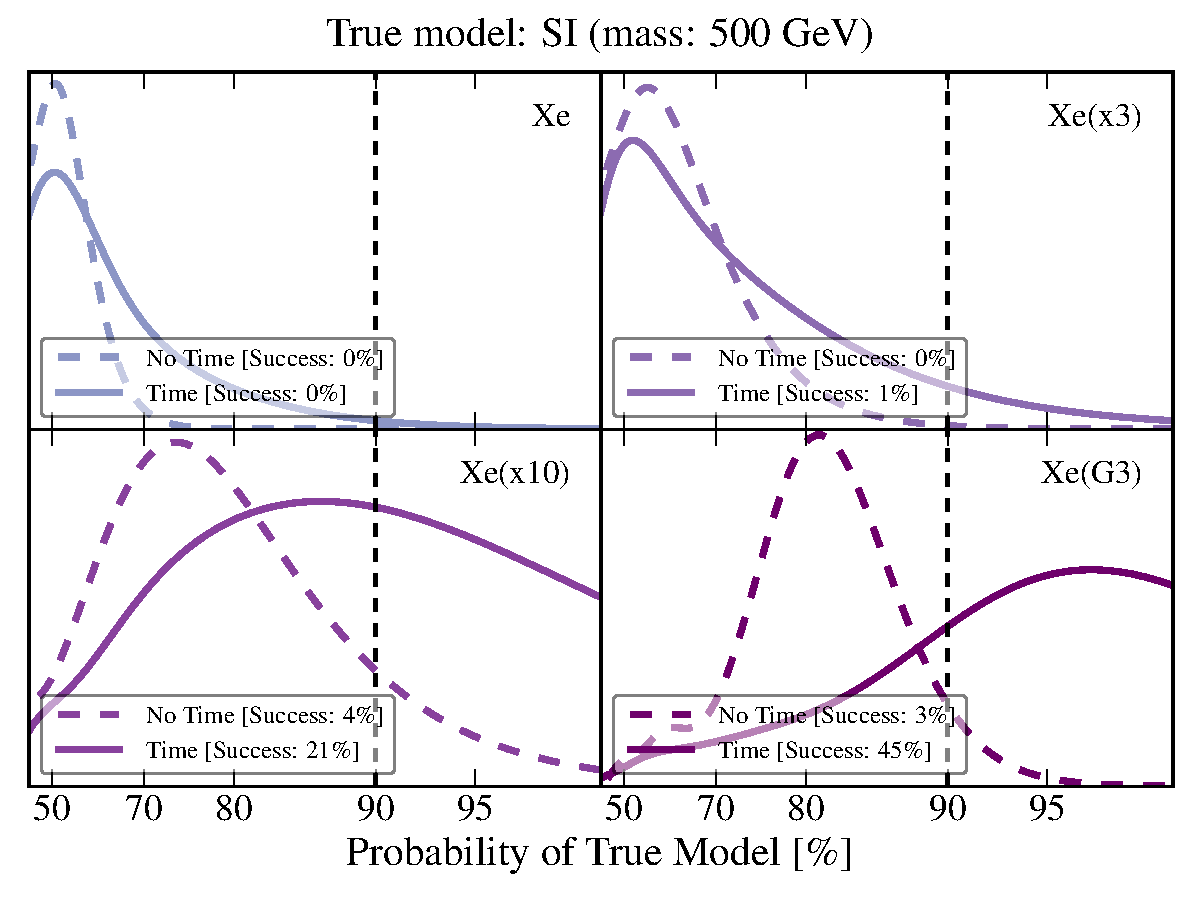
\includegraphics[width=0.7\textwidth]{plots/PDF_500GeV_SI_Higgs_50sims_Xe_Xe3x_Xe10x_XeG3_GF_TNT.pdf}
\caption{\label{fig:500gev_SI_Higgs_XeFull_TNT_GF}
Same as Fig.~\ref{fig:20gev_anapole_XeFull_TNT_GF} but for a $500$ GeV dark matter and the SI interaction.}
\end{figure*}

\bibliographystyle{JHEP}
\bibliography{mod-sel}

\end{document}